% document type
\documentclass[a4paper, twoside, openright]{report}
% character encoding
\usepackage[utf8]{inputenc}
% text encoding
\usepackage[T1]{fontenc}
% borders size
\usepackage[a4paper,top=2.5cm,bottom=2.5cm,left=3cm,right=3cm]{geometry}
% font size
\usepackage[fontsize=12pt]{scrextend}
% language of text
\usepackage[english]{babel}
% lingua per la bibliografia
\usepackage[fixlanguage]{babelbib}
% package per generare testo fittizio. Potrebbe essere
% utile nel controllare quanto un capitolo potrebbe essere
% grande e quindi quanto occupa nella pagina
\usepackage{lipsum}
% per ruotare le immagini
\usepackage{rotating}
% per modificare l'header delle pagine 
\usepackage{fancyhdr}
% per allineare in modo giustificato
\usepackage{ragged2e}
\justifying
% uso delle immagini
\usepackage{graphicx}
\usepackage{float}
% uso dei colori
\usepackage[dvipsnames, table]{xcolor}         
% uso dei listing per il codice
\usepackage{listings}          
% per inserire gli hyperlinks tra i vari elementi del testo 
\usepackage[colorlinks=true, allcolors=black]{hyperref}    
% diversi tipi di sottolineature
\usepackage[normalem]{ulem}
% package e comando per creare pagine vuote
\usepackage{afterpage}
\newcommand\blankpage{%
    \null
    \thispagestyle{empty}%
    \addtocounter{page}{-1}%
    \newpage
}
    
% package per creare comandi personalizzati
\usepackage{xpatch}
% package helper per le liste puntate
\usepackage{enumitem}
% package per l'utilizzo dei colori
% package per l'highlighting del codice
\usepackage{minted}
% package per gestire le caption
\usepackage{caption}
\usepackage{subcaption}
% per gestire tabelle su più pagine
\usepackage{longtable}
% per combinare le righe di una tabella
\usepackage{multirow}
% per creare i tree di directory
\usepackage{dirtree}
\setcounter{tocdepth}{4}

% per le icone a fianco dei titoli di sezione
\usepackage{etoolbox}
\newcommand{\icon}[1]{\includegraphics[height=12pt]{#1}}
\robustify{\icon}

\usepackage[absolute]{textpos}

\usepackage{amsmath}


\usepackage{booktabs}  % Per linee più eleganti (\toprule, \midrule)
\usepackage{array}     % Per una gestione avanzata delle colonne
\usepackage{url}
\usepackage{subcaption}
% 1. Per il disegno (l'ambiente tikzpicture)
\usepackage{tikz}

% 2. Per l'opzione [H] che forza la figura esattamente dove l'hai scritta
\usepackage{float}

\usepackage{pgfplots}
\pgfplotsset{compat=1.18} % Usa la versione più recente di pgfplots

\captionsetup[table]{labelformat=simple, labelsep=colon}


% Definizioni dei colori
\definecolor{colGreen}{RGB}{198, 224, 180}   
\definecolor{headBlue}{RGB}{189, 215, 238}   
\definecolor{headOrange}{RGB}{244, 176, 132} 
\definecolor{topRed}{RGB}{192, 0, 0}         
\definecolor{topGray}{RGB}{231, 230, 230}    

% Comandi personalizzati
\newcommand{\inv}[1]{\cellcolor{colGreen}\textbf{Invio #1}}
\newcommand{\ric}[1]{\cellcolor{colGreen}Ricevuto #1}
\newcommand{\rim}[1]{\cellcolor{colGreen}\textbf{\textcolor{red}{Rimosso #1}}}
\newcommand{\disc}{\cellcolor{colGreen}\textbf{\textcolor{red}{DISCONNESSIONE}}}

\usepackage{placeins}

\usepackage{changepage}
% -----------------------------------------------------------------

% Modifica lo stile dell'header
\pagestyle{fancy}
\fancyhf{}
\lhead{\rightmark}
\rhead{\textbf{\thepage}}
\fancyfoot{}
\setlength{\headheight}{15pt}

% Rimuove il numero di pagina all'inizio dei capitoli
\fancypagestyle{plain}{
  \fancyfoot{}
  \fancyhead{}
  \renewcommand{\headrulewidth}{0pt}
}

% comandi per cambiare temporaneamente la lingua
% abstract in inglese, al fine di cambiarne il titolo
\xpretocmd{\abstract}{\selectlanguage{english}}{}{} 
\xapptocmd{\endabstract}{\selectlanguage{italian}}{}{}

% formattazione e highlight del codice
\usemintedstyle{manni}
\setminted[python]{
    framesep=2mm,
    baselinestretch=1.2,
    fontsize=\ttfamily\footnotesize,
    linenos
}

% environment per impostare il codice in piu' pagine
\newenvironment{code}{\captionsetup{type=listing}}{}

% -----------------------------------------------------------------
\begin{document}

\begin{titlepage}
\begin{textblock*}{21cm}(0cm,13.66cm)
	\fontsize{20}{24}\selectfont
	\centerline  {\textbf{Embedded Operating Systems and Architectures}}
\end{textblock*}


\fontsize{14}{17}\selectfont

\begin{textblock*}{8cm}(12.33cm,23.55cm)
	\noindent	\textbf{Stridi Simone}
\end{textblock*}


\begin{textblock*}{21cm}(0cm,27.34cm)
	\centerline{Anno Accademico 2026/2027}
\end{textblock*}

\end{titlepage}
\afterpage{\blankpage}

\tableofcontents%\begin{adjustwidth}{0cm}{1.8cm}
%\makeatletter
%\@starttoc{toc}
%\makeatother
%\end{adjustwidth}

%\chapter{Introduction} \label{cap: Introduction}
\section{What is an Embedded Operating System?}
An \textbf{\textcolor{red}{operating system (OS)}} mediates \textbf{\textit{between application software and hardware}}. 
This \textbf{\textit{allows applications to request systems services, without needing to manually configure the hardware}}, like initialize the CPU, program timers, or handle raw hardware states.

In \textbf{\textcolor{red}{general-purpose systems (GPS)}}, the OS utilizes hardware like a \textbf{\textit{Memory Management Unit (MMU) to provide}} each application with its own \textbf{\textit{isolated virtual address space}}, preventing processes from interfering with the kernel or each other.

An \textbf{\textcolor{red}{Embedded Operating System (EOS)}}, by contrast, is a highly specialized, tightly constrained OS built into a larger device to execute one dedicated, fixed workload rather than general-purpose, user-installed software.

\begin{figure}[h]
    \centering
    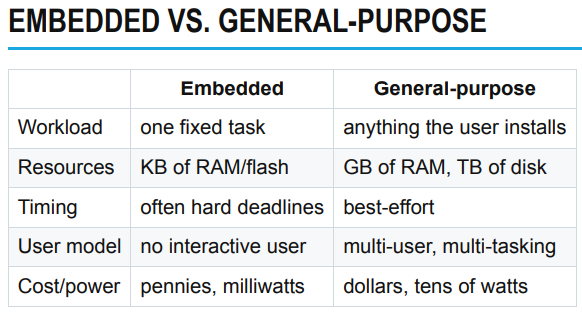
\includegraphics[width=0.5\linewidth]{contents/images/EvsGP.png}
    \caption{Embedded vs General Purpose OS}
\end{figure}

\textbf{\textcolor{red}{Properties: }}
\begin{itemize}
    \item \textbf{Resource Constraints}: It is engineered for \textbf{\textit{minimal overhead}}, operating within strict hardware limits of \textbf{\textit{kilobytes of SRAM (volatile-memory)}} and \textbf{\textit{Flash memory (persistent storage)}} (and operating on milliwatts of power) rather than gigabytes of RAM and massive storage drives.
    \item \textbf{Real-Time Determinism (RTOS)}: Many embedded OSes are Real-Time Operating Systems. This means \textbf{\textit{correctness depends}} not just on the logical output, but \textbf{\textit{on strict temporal deadlines}}. A result computed after its deadline (e.g., sampling a critical sensor every 1 ms) is considered a total system failure, prioritizing deterministic predictability over raw throughput.
    \item \textbf{Flat Memory Architecture}: Embedded OSes \textbf{\textit{frequently utilize a single, flat memory model}}. The startup code, kernel, drivers, and application tasks are all linked into one firmware image sharing a single physical address space, typically without MMU-enforced virtual memory or user-space protection.
    \item \textbf{Static Configuration}: Because the workload is known at compile time, \textbf{\textit{dynamic memory allocation is often replaced by static task counts and fixed buffers}}, and device drivers frequently rely on direct register access rather than heavily abstracted software layers.   
\end{itemize}

\subsection{Monolithic OS Structure}
A monolithic operating system structure is a design where \textbf{\textit{the entire operating system runs as a single, large program in kernel space}}, granting all components direct access to the computer's hardware and memory address space.

\begin{itemize}
    \item \textbf{Kernel Unito}: \textbf{\textit{All core services}}, such as process management, memory management, file systems, and device drivers, \textbf{\textit{live together inside the kernel}}.
    \item \textbf{Shared space}: \textbf{\textit{Every component shares the same memory space}}, meaning parts of the OS can talk to each other directly without message-passing protocols.
    \item  \textbf{Examples}: \textbf{\textit{Linux}} and traditional Unix systems use monolithic or modular-monolithic designs.
\end{itemize}

\begin{figure}[h]
    \centering
    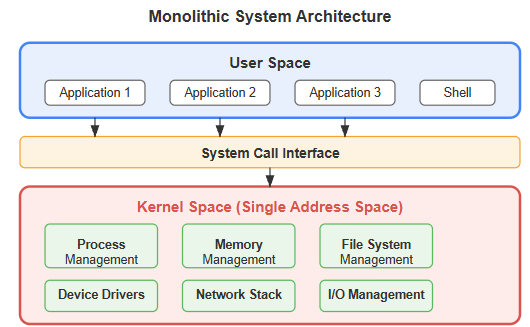
\includegraphics[width=0.8\linewidth]{contents/images/Monolithic.png}
    \caption{Monolithic Operating System Structure}
\end{figure}

\subsection{Microkernel OS Structure}
A microkernel structure is a\textbf{\textit{ minimalist operating system design that keeps only the absolute essential core mechanisms}}, such as low-level address space management, basic thread/process scheduling, and inter-process communication (IPC), in privileged supervisor/kernel mode.

 System services \textbf{\textit{are isolated independent modules, making it easier to update, replace, or unload components}} without rewriting or rebooting the whole system.
Or \textbf{\textit{if a service like a device driver fails, it won’t crash}} the whole system. Each service runs independently, so the core OS remains stable

\textbf{\textcolor{red}{Advantageous:}}
\begin{itemize}
    \item \textbf{Performance}: Because \textbf{\textit{the kernel only contains the essential functions}} required to manage the system, the microkernel design can improve performance. This \textbf{\textit{can make the system faster}} and more efficient.
    \item \textbf{Security}: The microkernel design can improve security by \textbf{\textit{reducing the system's attack surface}} by limiting the functions provided by the kernel. Malicious software may find it more difficult to compromise the system as a result of this.
    \item \textbf{Reliability}: Microkernels are \textbf{\textit{less complex than monolithic kernels}}, which can make them more reliable and less prone to crashes or other issues.
\end{itemize}

\begin{figure}[h]
    \centering
    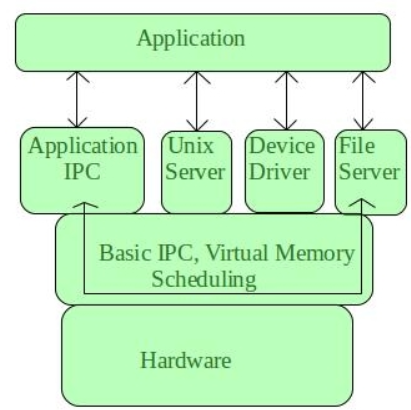
\includegraphics[width=0.5\linewidth]{contents/images/Microkernel.png}
    \caption{Microkernel Operating System Structure}
\end{figure}

\subsection{Flat OS Structure}
A flat structure operating system is an operating system design where \textbf{\textit{components are not separated into rigid hierarchical layers or isolated microkernel spaces, allowing programs to interact closely with or directly access underlying hardware and system services}}.

\textbf{\textcolor{red}{Properties: }}
\begin{itemize}
    \item \textbf{Single Linked Image}: The startup initialization code, the operating system kernel, device drivers, and \textbf{\textit{all application tasks are compiled and linked together into one single executable firmware image stored}} in \textbf{\textcolor{red}{Flash memory}}. There is no process loader dynamically launching separate applications at runtime.
    \item \textbf{Shared Memory}: There is \textbf{\textit{NO virtual-memory translation}} (like an MMU provides in desktop systems). The kernel, all tasks, and device peripherals map \textbf{\textit{directly to the same flat physical memory addresses}}, meaning all components can address the exact same RAM.
    \item\textbf{ No Hardware Isolation}: There is usually \textbf{\textit{no hardware-enforced boundary}} (such as user space versus kernel space) between different tasks.
    \item \textbf{Direct Execution}: \textbf{\textit{Tasks cooperate directly and rapidly through the scheduler and shared memory}}, rather than relying on complex, heavily abstracted inter-process communication.
\end{itemize}       

\textbf{\textcolor{red}{Advantages: }}
\begin{itemize}
    \item \textbf{High Speed}: Offers fast performance because there are fewer operational layers or communication bottlenecks.
    
    \item \textbf{Simple Development}: Easier for programmers to build and manage initially without complex boundary definitions.
\end{itemize}    

\textbf{\textcolor{red}{Disadvantages:}}
\begin{itemize}
    \item \textbf{Vulnerability}: \textbf{\textit{Lacks robust hardware protection and process isolation}}, meaning a single application failure or malicious program can crash the entire system.
    
    \item \textbf{Poor Scalability}: Becomes \textbf{\textit{difficult to maintain, expand}}, or debug as the system grows larger and more complex.
\end{itemize} 

\textbf{\textcolor{red}{Flat Firmware}}
Flat embedded firmware is an architecture where \textbf{\textit{the entire operating system and all applications reside in a single executable image}} operating \textbf{\textit{within one physical address space}}.   

\textbf{Single linked image}: The startup code, kernel, device drivers, and application tasks \textbf{\textit{are all compiled and linked together into one firmware image stored in Flash memory}}.
Tasks cooperate through shared memory and the scheduler.
There is \textbf{no process loader}, \textbf{no virtual-memory translation}, and usually \textbf{no hardware-enforced boundary between tasks}.

\textbf{\textcolor{red}{Flat firmware risks:}}
\begin{itemize}
    \item A simple programming error like \textbf{\textit{a bad pointer in an application task can overwrite}} and corrupt any writable state in the system, \textbf{\textit{including the OS kernel}}.
    
    \item A \textbf{\textit{blocked high-priority task can completely}} halt other important services, effectively \textbf{\textit{freezing the device}}.
\end{itemize}


\subsection{What we will do in the course?}
The \textbf{starting point (scratch-os)}: The course deliberately begins by having you build scratch-os, \textbf{\textit{which utilizes a "flat" firmware architecture}}. This is the simplest possible point on the spectrum. It \textbf{\textit{makes the entire internal pipeline}}, from the initial boot process to task scheduling, \textbf{\textit{completely visible}} and easy to understand.   

\textbf{The Transition (FreeRTOS)}: Later in the course, you will transition to using FreeRTOS. This system is \textbf{\textit{closer to a minimal, microkernel-flavored Real-Time Operating System (RTOS)}}. It features a small dedicated kernel and \textbf{\textit{implements real scheduling policies}}, but it is important to note that, by default, it still does not enforce memory protection between different tasks. 

FreeRTOS provides established, production-ready implementations of the core mechanisms you first build from scratch, such as task creation, priorities, timer-driven scheduling, queues, semaphores, mutexes, and interrupt-to-task communication. The primary reason for this two-step approach is educational: \textbf{\textit{using a high-level RTOS API call becomes much easier to reason about when you already understand the invisible state transitions happening underneath it}}. 

The \textbf{\textcolor{red}{pipeline}} you quoted represents the exact \textbf{\textcolor{red}{sequence of core mechanisms}} you will learn to build manually:

\begin{enumerate}
    \item \textbf{Reset}: Handling the initial hardware state upon powering up.
    
    \item \textbf{Initialise memory}: Setting up the RAM (copying and zeroing data) so C code can safely execute.
    
    \item \textbf{Start application}: Transitioning control to your actual application logic.
    
    \item \textbf{React to events and Schedule tasks}: Handling hardware interrupts and deciding which software task gets CPU time next.
    
    \item \textbf{Synchronise shared resources}: Ensuring that multiple tasks don't corrupt data when accessing the same memory or peripherals.
\end{enumerate}

The main takeaway is that you must build and understand these foundational mechanisms yourself before relying on a production RTOS API. 

\section{Microcontroller (MCU)}
A \textbf{microcontroller (MCU)} \textbf{\textit{integrates onto a single chip the components}} that a desktop computer typically splits across an entire motherboard. It operates as a self-contained system containing:
\begin{itemize}
    \item \textbf{CPU core}: The processor that executes instructions, such as the \textbf{\textit{ARM Cortex-M3}}.
    
    \item \textbf{SRAM}: Volatile \textbf{\textit{working memory}}, which is usually limited to tens of kilobytes.
    
    \item \textbf{Flash}: \textbf{\textit{Non-volatile program storage}} that allows code to run directly from it.
    
    \item \textbf{Peripherals}: \textbf{\textit{Built-in hardware interfaces}} like timers, UART, GPIO, and ADCs.
\end{itemize}

\textbf{\textcolor{red}{Microcontroller VS General-Purpose CPU}}
\begin{itemize}
    \item \textbf{Integration}: \textbf{\textit{A general-purpose desktop CPU is just the processing core}}; \textbf{\textit{it must use external buses}} to reach separate chips for RAM, storage, and I/O. An \textbf{\textit{MCU has all of these elements built}} directly into the \textbf{\textit{same chip}}.   
    
    \item \textbf{Memory Management}: A desktop CPU utilizes a Memory Management Unit \textbf{\textit{(MMU) to give}} every running process its own \textbf{\textit{isolated virtual address space}}. \textbf{\textit{An MCU}} relies on one flat physical address map shared by the code, data, and every peripheral register, meaning it \textbf{\textit{has no virtual memory and no MMU}} (a Cortex-M relies at most on an optional Memory Protection Unit).   
    
    \item \textbf{Hardware Interaction}: On an MCU, "the hardware" is simply memory that you write to directly. \textbf{\textit{Unlike general-purpose systems, there is no abstraction or driver layer}} sitting between your code and a device register.
\end{itemize}

\section{From Hardware To Software}
\subsection{QEMU (Virtual Hardware)}
\begin{itemize}
    \item Cos'è: QEMU è un emulatore software in esecuzione sul tuo computer (l'host) che simula fisicamente il comportamento di una specifica scheda a microcontrollore ARM (il target).   
    
    \item A cosa serve: Invece di costringerti a comprare e cablare una vera scheda elettronica, QEMU ti fornisce un ambiente identico e riproducibile (la macchina mps2-an385) su cui caricare e testare il tuo firmware. È la "finta" CPU ARM Cortex-M3 su cui girerà tutto il tuo codice. 
\end{itemize}

\subsection{Scratch-OS}
\begin{itemize}
    \item Cos'è: È un piccolissimo sistema operativo flat (piatto) che costruirete voi stessi da zero durante la prima parte del corso.  
    
    \item A cosa serve: Serve a svelare tutta la "magia invisibile" che c'è dietro ai sistemi operativi. L'obiettivo di scratch-os è farti scrivere a mano tutti quei meccanismi fondamentali che un OS normalmente nasconde: gestire il reset, inizializzare la RAM, reagire agli interrupt hardware e creare un basilare scheduler per far girare più task. 
\end{itemize}

\subsection{FreeRTOS}
\begin{itemize}
    \item Cos'è: È un vero e proprio Real-Time Operating System (RTOS) utilizzato nell'industria, basato su un'architettura più vicina a un microkernel.   
    
    \item A cosa serve: Una volta capito come si costruisce un OS (grazie a scratch-os), nella seconda parte del corso butterete via il vostro kernel manuale e inizierete a usare FreeRTOS. Questo vi permetterà di usare API standard e professionali per creare task, gestire priorità, code e semafori. Usare FreeRTOS diventerà facilissimo proprio perché, avendo costruito prima scratch-os, saprai esattamente cosa succede "sotto il cofano" a livello di registri e memoria. 
\end{itemize}

\subsection{mps2-an385}
mps2-an385 è il modello esatto di scheda che QEMU sta simulando. La scheda definisce la "mappa" del sistema: dice a QEMU che la memoria Flash parte dall'indirizzo 0x00000000, la SRAM da 0x20000000 e che ci sono specifiche periferiche (come l'output seriale) a determinati indirizzi.

The mps2-an385 machine board structure represents an ARM V2M-MPS2 (Cortex-M Prototyping System 2) motherboard configured via Application Note AN385. In this implementation, the ARM Cortex-M3 processor core and its primary system design kit (CMSDK) peripherals are synthesized within the board's onboard FPGA.

\subsection{ARM Cortex-M3}
L'ARM Cortex-M3 è un core di processore RISC a 32 bit progettato da ARM Holdings specificamente per applicazioni embedded a basso costo, bassa potenza e ad alte prestazioni.
\begin{figure}
    \centering
    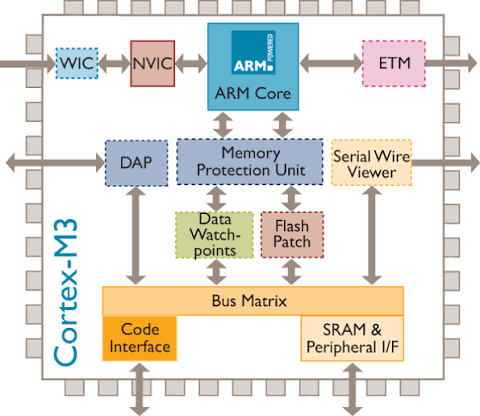
\includegraphics[width=0.5\linewidth]{contents/images/Cortex_M3.png}
    \caption{ARM Cortex-M3 microcontroller}
\end{figure}









\section{Machine Model}
\subsection{Cortex-M3 at Reset step}
When the \textbf{Cortex-M3} processor \textbf{\textit{is powered on}} or reset, it does not look for or discover an operating system. 

The sequence \textbf{\textit{involves two pointers}} (32-bit values) and it happens \textbf{\textit{entirely in hardware}} (directly readed from the vector table located in the Flash, \textbf{\textit{typically address 0x00000000}} is where the \textbf{vector table} is stored.) \textbf{\textit{before}} a single line of \textbf{\textit{your software is executed}}.

Those 2 lines provide the absolute minimum orientation it needs to function: a place to temporarily store data (RAM) and a place to start reading instructions (Flash).

\begin{enumerate}
    \item \textbf{Main Stack Pointer}: Tells the \textbf{\textcolor{red}{CPU's internal Stack Pointer register}} exactly where the top of the stack is located in the \textbf{\textit{SRAM (volatile memory)}}.
    \item \textbf{Reset Handler Address}: provides the initial value for the \textbf{\textcolor{red}{Program Counter}}, pointing it directly to a specific address in the \textbf{\textit{Flash memory (non-volatile memory)}} where your boot code lives.
\end{enumerate}

Once these two pointers are read, \textbf{\textit{the automated hardware boot phase is complete}}. The hardware hands over control to your software (the Reset\_Handler), which now relies on the newly established stack to prepare the C runtime environment and \textbf{\textcolor{red}{ultimately call your main() function}}.

\textbf{\textcolor{red}{CPU working on registers}}
The CPU operates on values held in registers. Memory is accessed explicitly
with load and store instructions.

\begin{figure}[h]
    \centering
    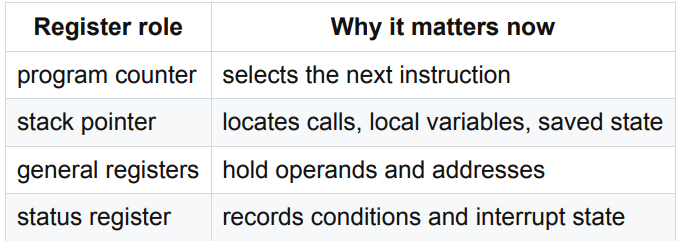
\includegraphics[width=0.8\linewidth]{contents/images/registers.png}
    \caption{Most used registers of ARM Cortex-M3}
\end{figure}

\subsection{Components}
Flash vs SRAM (Static RAM) roles:
\begin{itemize}
    \item \textbf{Flash Memory}: This is \textbf{\textit{non-volatile storage}}. It permanently stores the vector table, \textbf{\textit{the executable instructions}} (\textcolor{red}{.text section}), read-only \textbf{\textit{constants}} (\textcolor{red}{.rodata}), and the \textbf{\textit{initial byte values}} required for your initialized variables (\textcolor{red}{the initial .data image}).  
    
    \item \textbf{SRAM (Static RAM)}: This is fast, volatile working memory. It holds the actively used \textbf{\textit{initialized variables}} (\textcolor{red}{.data}), the \textbf{\textit{zero-initialized variables}} (\textcolor{red}{.bss}), the \textbf{\textit{heap area, and the stack}}.   
    
    \item \textbf{The Startup Requirement}: Because SRAM forgets everything when the system restarts, your custom \textbf{\textit{startup code must physically copy the initial values}} for the \textcolor{red}{.data} section \textbf{\textit{from Flash into SRAM}}, and explicitly clear the \textcolor{red}{.bss} section to zero before standard C code can safely execute.
\end{itemize}

\begin{figure}[h]
    \centering
    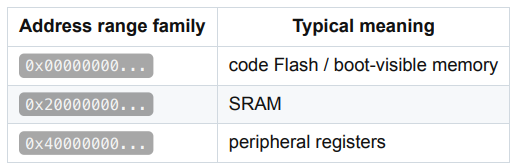
\includegraphics[width=0.8\linewidth]{contents/images/Memory_Addresses.png}
    \caption{Memory addresses begin}
\end{figure}

\textbf{Load/Store Architecture}: The Cortex-M3 executes a load/store instruction set. \textbf{\textit{To process data}}, a \textbf{\textcolor{red}{load instruction}} must bring the value from a specific memory address into a register, and a \textbf{\textcolor{red}{store instruction}} must \textbf{\textit{write}} the computed result \textbf{\textit{back to memory}}.

\begin{figure}[h]
    \centering
    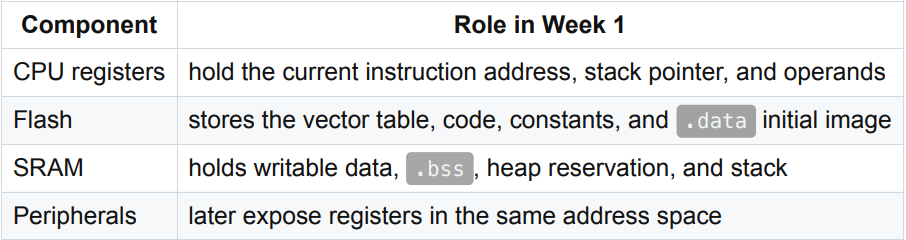
\includegraphics[width=0.85\linewidth]{contents/images/devices.png}
    \caption{Roles of each component inside the Cortex-M3}
\end{figure}













\chapter{Introduction to Embedded Systems and Toolchain}

\section{The Chain of Evidence and the Bare-Metal Toolchain}
Building a bare-metal firmware relies on a strict \textbf{chain of evidence}. Every tool in the build pipeline has a specific, essential job to connect your C source code to the physical hardware. 

Here is exactly what each component does in practice:

\begin{itemize}
    \item \textbf{Cross-Compiler (e.g., \texttt{arm-none-eabi-gcc}):} Your PC cannot run microcontroller code. The cross-compiler's job is to translate your human-readable C code into the exact binary language that the target CPU understands (for the Cortex-M3, this is the \textbf{Thumb-2} instruction set).
    
    \item \textbf{Linker and Linker Script (\texttt{.ld}):} The compiler creates isolated blocks of code, but the CPU needs them placed at specific physical addresses. The linker glues these blocks together, using the \textbf{linker script} as a map. It dictates that executable code and constants must be saved in permanent \textbf{Flash} memory, while writable variables must be placed in volatile \textbf{SRAM}.
    
    \item \textbf{Hardware Vector Table:} A fixed directory located at the very beginning of the memory (address \texttt{0x00000000}). When powered on, the CPU is "blind" and reads the first two entries here to know how to start:
    \begin{enumerate}
        \item The first word tells the CPU where to place its temporary working memory (the \textbf{Main Stack Pointer}).
        \item The second word tells the CPU the exact address of the first instruction to execute (the \textbf{Reset Handler}).
    \end{enumerate}
    
    \item \textbf{Startup Code (Reset Handler):} A crucial piece of code that runs \textit{before} your \texttt{main()} function. Its job is to "prepare the house" (the RAM) for your application. It performs two critical tasks:
    \begin{enumerate}
        \item \textbf{Data Initialization:} It copies variables that have a starting value (e.g., \texttt{int x = 5;}, the \texttt{.data} section) from the permanent Flash into the working SRAM.
        \item \textbf{BSS Clearing:} It fills variables that have no starting value (the \texttt{.bss} section) with zeros directly in SRAM.
    \end{enumerate}
    Only after the RAM is perfectly set up, the startup code safely calls \texttt{main()}.
\end{itemize}

Understanding what each component actually does transforms debugging. If a program crashes before even reaching \texttt{main()}, a developer immediately knows to check the linker script or the startup code, rather than the application logic.

\section{What is an Embedded Operating System?}
An operating system (OS) manages hardware resources for applications. General-Purpose OS use a Memory Management Unit (MMU) to isolate applications in virtual memory. 

An \textbf{Embedded Operating System (EOS)} is completely different: it is a highly specialized, tightly constrained OS built to execute a single, fixed workload on a specific hardware device.

\subsection{Key Properties of Embedded Systems}
\begin{itemize}
    \item \textbf{Resource Constraints:} Built for kilobytes of RAM/Flash and milliwatts of power. Zero overhead allowed.
    \item \textbf{Real-Time Determinism (RTOS):} Deadlines matter as much as logic. A correct calculation delivered late (e.g., in an airbag sensor) is a total system failure. Predictability beats raw speed.
    \item \textbf{Flat Memory Architecture:} No virtual memory. The kernel, drivers, and tasks share one physical address space and are compiled into a single firmware image.
    \item \textbf{Static Configuration:} Since the workload is fixed at compile time, dynamic memory allocation (\texttt{malloc}) is rarely used. Tasks, memory pools, and hardware resources are statically allocated.
\end{itemize}

\begin{figure}[h]
    \centering
    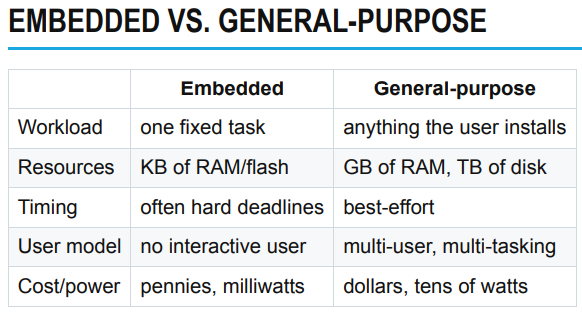
\includegraphics[width=0.4\textwidth]{contents/images/EvsGP.png}
    \caption{Embedded vs General Purpose OS characteristics.}
\end{figure}

\section{Operating System Architectures}

\subsection{Monolithic OS Structure}
The entire operating system runs as a single, large program in a privileged kernel space.
\begin{itemize}
    \item \textbf{Unified Kernel:} Core services (scheduling, memory, file systems, drivers) live together.
    \item \textbf{Maximum Throughput:} Components share the same memory and communicate directly without message-passing overhead.
    \item \textbf{The Risk:} If one driver crashes, the entire system halts (e.g., Linux, Windows).
\end{itemize}

\begin{figure}[h]
    \centering
    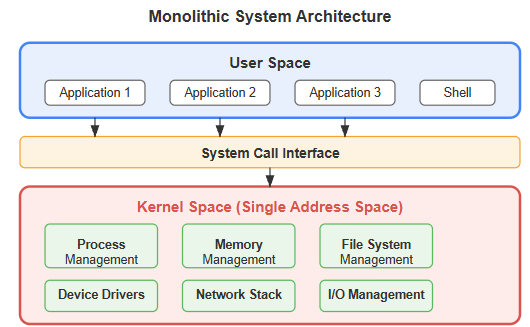
\includegraphics[width=0.3\textwidth]{contents/images/Monolithic.png}
    \caption{Monolithic Operating System Structure.}
\end{figure}

\subsection{Microkernel OS Structure}
A minimalist design that keeps only essential features (scheduling, basic memory management, IPC) in privileged mode. Everything else runs as isolated user-space apps.
\begin{itemize}
    \item \textbf{Fault Containment (Advantage):} High security and reliability. If a device driver crashes, it restarts independently without bringing down the core OS.
    \item \textbf{Performance Penalty (Disadvantage):} Slower than monolithic systems. Isolated components must constantly talk via Inter-Process Communication (IPC), causing heavy context-switching overhead.
\end{itemize}

\begin{figure}[h]
    \centering
    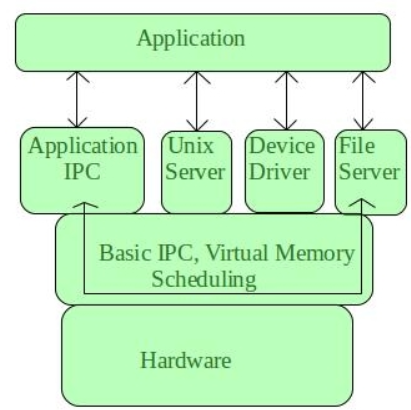
\includegraphics[width=0.3\textwidth]{contents/images/Microkernel.png}
    \caption{Microkernel Operating System Structure.}
\end{figure}

\subsection{Flat OS Structure (Bare-Metal)}
The simplest architecture, where there are no layers or isolated spaces.
\begin{itemize}
    \item \textbf{Single Linked Image:} The startup code, OS kernel, device drivers, and apps are merged into one executable stored in Flash. No dynamic app loader.
    \item \textbf{Raw Physical Memory:} Everything maps directly to raw physical addresses. No MMU translation.
    \item \textbf{No Hardware Isolation:} No protection boundaries between kernel and user space.
\end{itemize}

\textbf{Advantages:}
\begin{itemize}
    \item \textbf{High Speed:} Zero latency from OS abstractions or IPC.
    \item \textbf{Simplicity:} Easy to build and deploy for small, dedicated hardware.
\end{itemize}

\textbf{Disadvantages \& Risks:}
\begin{itemize}
    \item \textbf{Zero Isolation:} A single bug (e.g., a bad pointer) in any task can overwrite the entire system memory and cause a hard crash.
    \item \textbf{Blocking Tasks:} A stuck function or infinite loop halts the entire CPU.
    \item \textbf{Poor Scalability:} Unmanageable as code complexity grows.
\end{itemize}


\subsection{What we will do in the course?}
\textbf{The starting point (\textit{scratch-os}):} The course begins by building \textit{scratch-os}, which utilizes a \textbf{\textit{flat firmware architecture}}. This exposes the entire internal pipeline, from the initial boot process to task scheduling, making the hardware assumptions completely visible and non-negotiable.

\textbf{The transition (FreeRTOS):} Later, we transition to FreeRTOS, a production-ready RTOS closer to a microkernel philosophy. It features a small dedicated kernel and implements real scheduling policies (though, by default, it does not enforce memory protection). The educational goal is clear: \textbf{\textit{using a high-level RTOS API is easy only when you already understand the invisible state transitions happening underneath it}}.

The exact \textbf{\textcolor{red}{sequence of core mechanisms}} you will build manually:
\begin{enumerate}
    \item \textbf{Reset}: Handling the initial hardware state upon power-up.
    \item \textbf{Initialize memory}: Setting up the RAM (copying `.data`, zeroing `.bss`) so C code can safely execute.
    \item \textbf{Start application}: Transitioning control to the application logic.
    \item \textbf{React to events \& Schedule}: Handling hardware interrupts and deciding which task gets CPU time next.
    \item \textbf{Synchronize}: Ensuring tasks do not corrupt shared data or peripherals.
\end{enumerate}

\section{The Target Machine: Cortex-M3 and QEMU}
Embedded software is built for a known processor and a fixed memory map. It cannot rely on an OS to create a process, assign an address space, or arrange standard I/O. 

\subsection{Microcontroller (MCU) vs General-Purpose CPU}
A \textbf{microcontroller (MCU)} integrates onto a single chip the components that a desktop computer splits across a motherboard.
\begin{itemize}
    \item \textbf{Integration}: A desktop CPU is just a processing core requiring external buses for RAM and I/O. An MCU has the CPU, RAM, Flash, and Peripherals (Timers, UART, GPIO) built directly into the same chip.
    \item \textbf{Memory Management}: Desktop CPUs use an MMU to provide isolated virtual address spaces. An MCU relies on a \textbf{\textit{single flat physical address map}} shared by code, data, and peripherals (No MMU).
    \item \textbf{Hardware Interaction}: On an MCU, hardware is simply memory you write to directly. There is no abstraction layer between your code and a device register.
\end{itemize}

\subsection{The QEMU target (\texttt{mps2-an385})}
Instead of physical hardware, the course uses \textbf{QEMU}, a software emulator. Specifically, it targets the \texttt{mps2-an385} machine, which models an \textbf{ARM Cortex-M3} processor. The linker script strictly defines its physical memory map:
\begin{itemize}
    \item \textbf{FLASH (Origin: \texttt{0x00000000}, 4 MiB):} Non-volatile. Holds the initial image: vector table, executable instructions (`.text`), and read-only constants (`.rodata`).
    \item \textbf{SRAM (Origin: \texttt{0x20000000}, 4 MiB):} Volatile. Holds mutable state: initialized globals (`.data`), zero-initialized globals (`.bss`), the heap, and the stack. 
    \item \textbf{The Stack:} It starts at the very top of the RAM (\texttt{0x20400000}) and \textbf{\textit{grows downwards}} to lower addresses.
\end{itemize}

\subsection{Peripheral Registers and the \texttt{volatile} Keyword}
In later weeks, device drivers will interact with peripherals by reading/writing to fixed memory addresses. These memory accesses MUST be declared \textbf{\texttt{volatile}} in C. 
\begin{itemize}
    \item \textbf{Why \texttt{volatile}?}: It tells the compiler that the value at that memory address can change outside the program's control (e.g., a hardware sensor updating), or that a write triggers a physical effect. Without \texttt{volatile}, the compiler's optimizer might delete the memory access, assuming it's an unused ordinary variable. 
    \item \textit{Note:} \texttt{volatile} does \textbf{not} provide atomicity or concurrency protection; it only ensures the access is physically executed by the CPU.
\end{itemize}







\section{Technical Foundations \& Toolchain}

\subsection{From Source Code to a Running Program}
The goal of this phase is to understand how to compile and run an application step by step, working directly with commands without relying on an IDE (like Visual Studio Code). Often, development environments hide the real compilation process behind a simple "Play" button, but when developing operating systems, it is essential to understand what actually happens under the hood.

The toolchain is a pipeline composed of several small tools, where the output of one becomes the input of the next:
\begin{itemize}
    \item \textbf{C Preprocessor:} manages and expands directives like \texttt{\#include} and \texttt{\#define}.
    \item \textbf{Compiler:} takes the preprocessed code and generates assembly code (\texttt{.s}).
    \item \textbf{Assembler:} converts the assembly into machine code, producing object files (\texttt{.o}).
    \item \textbf{Linker:} concatenates matching sections, resolves symbols to final addresses, and through an \texttt{.ld} script, generates the final binary image (the ELF image).
\end{itemize}

% \includegraphics[width=0.8\textwidth]{images/toolchain_pipeline.png}
% Suggested caption: Toolchain pipeline from C source to ELF image

\subsection{Why Cross-Compilation?}
Developing for embedded systems introduces an architectural problem: the computer we are writing the code on (Host) is different from the machine where the code will be executed (Target)[cite: 1]. The host is typically an x86-64 or Apple Silicon machine, whereas our target is an ARM Cortex-M3 processor[cite: 1].

A normal \texttt{gcc} compiler installed on the computer emits code optimized for the machine it runs on, which makes it useless for our purpose[cite: 1]. For example, a recent Mac's native compiler would generate code for a 64-bit ARM architecture, while our target board requires code for a 32-bit ARM architecture.

For this reason, a \textbf{cross-compilation toolchain} (specifically \texttt{arm-none-eabi-*}) is required[cite: 1]. It runs on the host but generates code for the target's ISA (Instruction Set Architecture)[cite: 1].

The \texttt{none-eabi} nomenclature is crucial to understand the environment we are working in:
\begin{itemize}
    \item \textbf{none:} indicates the absence of a host operating system on the target (bare-metal development)[cite: 1].
    \item \textbf{eabi:} indicates the use of the standard embedded ARM ABI (Application Binary Interface)[cite: 1].
\end{itemize}

Working in a "bare-metal" environment means not having the standard libraries typical of desktop operating systems: there will be no \texttt{printf} to a console, no \texttt{malloc} dynamic allocation supported by an OS, and no \texttt{\_start} function from a C library unless we explicitly provide it[cite: 1].

\subsubsection{Checking the Toolchain: Host vs Target}
To concretely verify the difference between compilers, we can simply query the toolchain from the terminal:
\begin{itemize}
    \item By running \texttt{gcc -dumpmachine}, you get the architecture of your host machine (e.g., a 64-bit architecture for a recent desktop system)[cite: 1].
    \item By running \texttt{arm-none-eabi-gcc -dumpmachine}, the output will clearly indicate a 32-bit ARM architecture followed by the \texttt{none} environment.
\end{itemize}

Getting two completely different target strings for the same command typed on the same computer demonstrates the fundamental concept of a cross toolchain[cite: 1]. When writing an operating system from scratch, it is imperative to use this type of compiler, generate the binary file, transfer it to the target machine, and finally run it.


\subsection{Host, Target, and Emulator}
During the development of software for embedded systems, it is essential to keep three key roles distinct in the compilation and testing process[cite: 1]:
\begin{itemize}
    \item \textbf{Host:} This is the PC we work on (e.g., our laptop) and where the text editor, toolchain, and other development tools are executed[cite: 1].
    \item \textbf{Target:} This is the physical hardware destination machine (in our case, a board with an ARM Cortex-M3 processor) for which the executable (the ELF image) is generated[cite: 1].
    \item \textbf{Emulator:} This is a virtual machine that simulates the target's hardware via software directly on our host[cite: 1]. In our case, lacking the physical board, we will use \textbf{QEMU} to test the execution of the programs[cite: 1].
\end{itemize}

\subsection{Reset Code and the Transition to C}
When running a program on a desktop computer, the operating system and the C runtime take care of preparing the memory and starting the program automatically[cite: 10]. In a bare-metal environment, at boot time, no such service exists[cite: 10]. 

To execute even just the first instruction of our \texttt{main()} function, it is necessary to have startup code (\texttt{boot/startup.c}) that acts as the bridge between the reset hardware and the application[cite: 10]. 

This code is responsible for making the C runtime's assumptions true before \texttt{main()} runs: it guarantees that every global variable already has its promised value (by initializing the \texttt{.data} and \texttt{.bss} memory sections) by the time \texttt{main()} starts[cite: 10].

The startup source also defines crucial bare-metal safety mechanisms:
\begin{itemize}
    \item \textbf{\texttt{Default\_Handler}:} An infinite loop used for unimplemented exception vectors. Stopping in that known loop is much safer and more diagnosable than falling into arbitrary memory after an unexpected hardware exception.
\end{itemize}

\subsection{Preprocessing: Assemble the Translation Unit}
When we start compiling (e.g., by typing the classic \texttt{gcc} command), the process is not monolithic but is divided into very distinct phases. The very first phase is handled by the \textbf{C preprocessor}. 
The preprocessor analyzes the C source code looking for directives (commands starting with the \texttt{\#} character, such as \texttt{\#include} or \texttt{\#define}) and expands these macros before the compiler actually sees the program[cite: 1]. 

This is purely text substitution, without any machine code generation[cite: 1]. For example, upon encountering an \texttt{\#include} command, the preprocessor locates the specified file and essentially "copies and pastes" it into the source file, replacing the original directive.
The result of this operation is a \textit{translation unit}: a single file of pure C code with all macros and headers already expanded[cite: 1].

\subsubsection{Try It: Preprocess Only}
We can instruct the toolchain to run \textit{only} the preprocessing phase by using the \texttt{-E} flag. The command to run in the terminal is the following[cite: 1]:

\texttt{arm-none-eabi-gcc -mthumb -mcpu=cortex-m3 -nostartfiles -ffreestanding -E src/main.c -o build/main.i}

In this string, we provide several options to describe to the toolchain the characteristics of the machine we actually have available[cite: 1]:
\begin{itemize}
    \item \texttt{-mthumb} and \texttt{-mcpu=cortex-m3}: these indicate, respectively, to use the Thumb instruction set and that the target CPU is a Cortex-M3[cite: 1].
    \item \texttt{-nostartfiles} and \texttt{-ffreestanding}: these signal that we are working in a bare-metal environment, meaning without standard operating system libraries or default startup files[cite: 1]. These options will be the default for our projects.
    \item \texttt{-E}: commands the compiler to stop immediately after preprocessing[cite: 1].
\end{itemize}

If we open the generated output file (\texttt{main.i}), we will notice fundamental changes compared to the original source:
\begin{enumerate}
    \item All text comments present in the source have been removed by the preprocessor.
    \item The \texttt{\#include <stdint.h>} directive has disappeared, entirely replaced by the expanded text (the typedef definitions) contained in that header file[cite: 1].
    \item The original C code of the \texttt{main()} function has remained textually identical at the bottom of the file[cite: 1].
\end{enumerate}
This demonstrates that the actual compiler, in subsequent steps, will never read our original \texttt{main.c}, but will work on this "translated" file (\texttt{main.i}), which can become huge if there are many files to include.

\subsection{Compilation: C Becomes Target Instructions}
Once preprocessing is finished, the compiler itself comes into play. The role of this step is to check the C syntax and translate the preprocessed code into \textbf{assembly} code specific to our target architecture[cite: 1]. 
All the options we provided earlier (such as \texttt{-mcpu}) are needed precisely by the compiler to know exactly which instructions to generate for 32-bit ARM microprocessors.

\subsubsection{Compilation and Target Architecture}
There are many 32-bit ARM microprocessors available, so it is necessary to specify the exact model being used, which in our case is the Cortex-M3. This specific CPU supports the Thumb instruction set (Thumb-2)[cite: 1]. Therefore, the compiler must be instructed precisely about the target CPU by providing specific options[cite: 1]. Finding the correct configuration involves matching the hardware datasheet specifications with the extensive GCC compiler documentation. Once the correct configuration is established and understood, it can be seamlessly applied to all future projects running on that same target machine.

\subsubsection{Try It: Stop After Compilation}
To observe the compilation phase without proceeding further in the pipeline, we can run the compiler using the \texttt{-S} flag (instead of the \texttt{-E} flag used for preprocessing)[cite: 1]. The \texttt{-S} option instructs the toolchain to run the preprocessor, compile the code, and stop immediately after producing the assembly version of the C program[cite: 1].
    
The output is typically stored in a file with a \texttt{.s} extension, such as \texttt{main.s}. Opening this file reveals that the original high-level C program has been translated into low-level ARM assembly instructions[cite: 1]. These instructions are written using human-readable mnemonics, not raw binary code, proving that the compiler's role at this specific stage is purely translation into assembly language[cite: 1]. While reading these files is not strictly required for this course, it is crucial to know that this intermediate translation step always takes place.

\subsection{Assembly: Instructions Become Relocatable Bytes}
Once the assembly version of the code is generated, the next tool in the chain is the \textbf{Assembler}. Its role is similar to a compiler, but it specifically takes the assembly code (\texttt{.s}) and translates it into binary machine code[cite: 1]. 

The output of this phase is an \textbf{object file} (identifiable by the \texttt{.o} extension). However, it is important to emphasize that the binary code contained in an object file is still not executable firmware[cite: 1]. Because projects are usually composed of multiple source files, the assembler processes each file in complete isolation. As a result, the generated object files contain machine-code bytes, section names, and symbol definitions, but they still lack proper, final memory addresses[cite: 1]. They may also contain unresolved references to code located in other object files (for instance, \texttt{startup.o} referring to \texttt{main}), which cannot be resolved at this stage[cite: 1].

\subsubsection{Try It: Assemble to an Object File}
To run the complete compiling chain up to the end of the assembly phase (executing preprocessing, compiling, and assembling sequentially), the \texttt{-c} flag must be used[cite: 1]. We can apply this to the different source files in our project:
\begin{itemize}
    \item \texttt{arm-none-eabi-gcc [...] -c boot/startup.c -o build/boot/startup.o}[cite: 1]
    \item \texttt{arm-none-eabi-gcc [...] -c src/main.c -o build/src/main.o}[cite: 1]
\end{itemize}

By doing this, we generate the object files \texttt{startup.o} and \texttt{main.o}. Unlike the previous \texttt{.i} and \texttt{.s} files, these object files represent the first output in the pipeline that is entirely in binary format[cite: 1]. Opening them with a standard text editor will reveal unreadable characters, as they are no longer in a human-readable format.


\subsubsection{Inspecting Object Files}
To understand what is inside an object file, we can use a tool provided by our toolchain called \texttt{arm-none-eabi-nm}[cite: 1]. This tool reads the \texttt{.o} files and extracts information in a human-readable way, specifically focusing on "symbols"[cite: 1]. 

Symbols represent the memory addresses that our program uses, which at this assembly stage are still left open and undefined[cite: 1]. For example, if we run the tool on our object files, we can look for the \texttt{main} function:
\begin{itemize}
    \item In \texttt{startup.o}, there is a call to the \texttt{main} function, but it is not defined there. The tool will label this symbol with a \textbf{U} (Undefined), meaning it is referenced but its address is unknown[cite: 1].
    \item In \texttt{main.o}, the function is actually written and defined. The tool will label this symbol with a \textbf{T} (indicating it is defined in the \texttt{.text} section)[cite: 1].
\end{itemize}
This separation is completely normal: the files are compiled in isolation, and it will be the linker's job to connect the "U" to the "T" and assign the final memory addresses[cite: 1].

\subsection{Linking: Creating the Executable}
As established, object files are not runnable firmware[cite: 1]. In ARM architecture, every assembly line corresponds to a 32-bit instruction with a fixed binary encoding. However, whenever an instruction needs to reference a memory address (like calling a function), those bits are left blank and filled with symbols instead. 

To convert these isolated objects into a final executable, we need a last step: the \textbf{Linker}[cite: 1]. The linker takes all the independent object files, concatenates matching sections, resolves every symbol to a final address, and patches all the references[cite: 1]. The output is an executable file formatted as \textbf{ELF} (Executable and Linking Format), which is the standard format originally designed in Unix and used globally (unlike the proprietary \texttt{.exe} format used by Windows)[cite: 1].

\subsubsection{The Linker Script}
When compiling a program on a standard PC, the operating system manages memory automatically, so the linker already knows what to do[cite: 1]. However, in a bare-metal embedded system, there is no operating system to rely on[cite: 1]. 

Therefore, we must explicitly instruct the linker on how to organize the different pieces of code in memory using a \textbf{Linker Script} (usually a \texttt{.ld} file)[cite: 1]. This script specifies the physical addresses of the hardware, detailing exactly what goes into the Flash memory (e.g., \texttt{.text}, \texttt{.rodata}) and what goes into the SRAM (e.g., \texttt{.data}, \texttt{.bss}, stack)[cite: 1]. Without this script, the toolchain wouldn't know the chip's specific memory map[cite: 1].

\subsubsection{Try It: Link the Objects}
If we want to run the compiler without stopping at intermediate steps and link the project, the command becomes more complex because we must include the linker script and all the necessary object files[cite: 1]. 

The command looks like this:
\texttt{arm-none-eabi-gcc [...] -T scripts/mps2\_m3.ld [...] build/boot/startup.o build/src/main.o -o build/scratch-os.axf}[cite: 1]

Here, the \texttt{-T} flag is crucial because it tells the compiler which linker script to use (\texttt{scripts/mps2\_m3.ld})[cite: 1]. After running this, we obtain our final, linked ELF image (\texttt{scratch-os.axf}). If we inspect it again with \texttt{arm-none-eabi-nm}, the \texttt{main} symbol will no longer be marked as "U" (undefined), but will have a finalized memory address assigned by the linker[cite: 1].


\subsubsection{The Linker Script and the Map File}
To perform the final link, the linker needs a strict description of physical memory[cite: 14]. To provide this, the link command in the Makefile uses specific flags assigned to the \texttt{LDFLAGS} variable:

\begin{lstlisting}[language=make]
LDFLAGS := -T scripts/mps2_m3.ld
LDFLAGS += -Xlinker -Map=build/output.map
\end{lstlisting}

\begin{itemize}
    \item \textbf{The Linker Script (\texttt{-T}):} The first option chooses the course linker script (\texttt{scripts/mps2\_m3.ld})[cite: 14]. The script begins by declaring the \texttt{FLASH} and \texttt{RAM} regions, then specifies the output sections that occupy them. Its internal syntax defines how it places the vector table so the processor finds it at reset, how it splits an initialized global's storage between a Flash load address and a RAM run address, and how it reserves the heap and stack. While writing this script from scratch is a Week 2 topic, for now, it is provided as-is to make the build work.
    
    \item \textbf{The Map File (\texttt{-Map}):} The second option emits a map file (\texttt{build/output.map})[cite: 14]. This file is an invaluable explanation of exactly where the linker placed each input contribution and symbol[cite: 14]. 
\end{itemize}

For Week 1, reading the generated map file is enough evidence that the script successfully assigned the final addresses and generated a valid executable binary file[cite: 14].

\subsection{The ELF Image and its Map}
The final target file generated by the toolchain is \texttt{build/scratch-os.axf}. The \texttt{.axf} suffix is commonly used for an ARM executable containing debug information, but the underlying file format is standard \textbf{ELF (Executable and Linkable Format)}[cite: 14, 15]. 

The ELF file organizes the program into several useful views[cite: 15, 16]:
\begin{itemize}
    \item \textbf{Sections:} Serve the linker and debugger (e.g., \texttt{.text}, \texttt{.rodata}, \texttt{.data}, \texttt{.bss})[cite: 15, 16].
    \item \textbf{Program Headers:} Describe memory ranges that a loader (or QEMU) places in memory[cite: 15].
    \item \textbf{Symbols:} Assign human-readable names to final physical addresses.
\end{itemize}

\subsubsection{Thumb State and The Entry Point}
The Week 1 build generates a 32-bit, little-endian ARM ELF executable. Running the command \texttt{arm-none-eabi-readelf -h -S build/scratch-os.axf} extracts the ELF header and reports the entry point at \texttt{0x49}[cite: 15]. 

However, looking at the map file, the \texttt{Reset\_Handler} is located at \texttt{0x00000048}. This mismatch is not an error: the low bit in the ELF entry address (\texttt{0x49} vs \texttt{0x48}) explicitly records the \textbf{Thumb state}. They describe the exact same execution entry, but the \texttt{+1} tells the CPU to execute in Thumb-2 mode.

\subsubsection{Sections Layout in Week 1}
The generated ELF contains the following allocated sections mapping directly to the physical addresses dictated by the linker script:

\begin{lstlisting}
.isr_vector  address 0x00000000  size 0x40
.text        address 0x00000040  size 0xa0
.data        address 0x20000000  size 0x0
.bss         address 0x20000000  size 0x0
.heap        address 0x20000000  size 0x1000
\end{lstlisting}

The map file (\texttt{build/output.map}) explicitly tracks this derivation[cite: 14]. It records the 64-byte vector table at Flash address zero, followed by the startup code (\texttt{startup.o}) at \texttt{0x40}. The application code (\texttt{main.o}) begins at \texttt{0xa4}, and the \texttt{"toolchain OK\char`\\n"} string literal is placed in \texttt{.rodata} at \texttt{0xd0}. 

\subsubsection{File Size vs RAM Usage}
In this specific Week 1 snapshot, the \texttt{.data} and \texttt{.bss} sections have a size of \texttt{0x0}. This should \textbf{not} be misread as evidence that RAM initialization is optional in bare-metal systems[cite: 10, 16]. It merely indicates that this specific, tiny program has no global variables needing those regions yet[cite: 16].

To accurately verify memory usage, developers run \texttt{arm-none-eabi-size build/scratch-os.axf}[cite: 17]. For Week 1, it reports 224 bytes of text, 0 bytes of data, and 4096 bytes of \texttt{bss}[cite: 17]. Note that this 4096-byte \texttt{bss} total includes the \texttt{.heap} section, deliberately reserved in the linker layout to occupy RAM[cite: 17].
\subsection{Debug Information for Host Tools}
When an operating system is finalized and released, information about the original source code is typically stripped from the binary to reduce size and protect intellectual property. However, during development and debugging, it is highly beneficial to generate binary files that contain debugging information[cite: 48]. 

Specific compiler options can embed source-level debug metadata inside the ELF[cite: 48]. This does not mean the target machine understands C; it still only runs machine instructions[cite: 48]. Instead, this metadata allows host-side tools (like QEMU or a debugger) to associate a specific binary instruction address with a corresponding C file line, function, or variable[cite: 48]. This bridge between high-level C code and low-level execution makes investigating crashes possible without altering the basic boot image[cite: 48].

\subsection{What Make Actually Does}
While it is crucial to understand how to compile an embedded program manually, step by step, doing so in practice is extremely inefficient[cite: 49]. Remembering every compiler flag, every linker script option, and listing every single C file becomes impossible for complex projects (for instance, the FreeRTOS kernel consists of hundreds of C files)[cite: 49]. 

To automate the compilation process, we use tools like \textbf{Make}, which is the standard toolchain automation used by Linux and FreeRTOS[cite: 49]. A \texttt{Makefile} is essentially a text-based script that defines a set of rules to compile many files[cite: 49]. 

\subsubsection{Targets Model Desired Outcomes}
The \texttt{Makefile} works by defining \textbf{targets} and the actions required for each target[cite: 50]. A target is a named file or action that Make knows how to produce[cite: 50]. For example, if you have a target named \texttt{all}, you can simply type \texttt{make all} in the terminal, and the tool will execute all the instructions associated with that target[cite: 50]. Some targets, like \texttt{clean} or \texttt{run}, are usually actions rather than actual files, and they are declared as \texttt{.PHONY} to prevent conflicts with a same-named file[cite: 50].

Make is also powerful because it tracks \textbf{prerequisites} (the dependency graph)[cite: 50, 54]. If you specify that the linking step requires all object files to be created first, Make will search for the rule to generate those object files if they do not exist[cite: 50, 54]. It works backward, starting from the desired result and executing all the necessary preceding steps[cite: 50, 54].

\subsubsection{Prerequisites Capture Rebuild Logic}
Another key feature of Make is its ability to rebuild a target only if a prerequisite is newer than the target itself[cite: 49, 51]. For example, if you change one variable in a massive project (like the Linux kernel, which can take hours to compile), you do not want to recompile everything[cite: 49, 51]. Make identifies that only one \texttt{.c} file has changed, recompiles that specific file into an object file, and then simply re-runs the linker to update the final ELF image[cite: 49, 51].

To identify if something has changed, Make uses the last modified timestamp of the files[cite: 51]. However, this can sometimes lead to issues. If you are using version control (like Git) or syncing folders via cloud services (like OneDrive or Dropbox), file timestamps can become corrupted or mistakenly set in the future. In these cases, you might modify a file, but Make will refuse to recompile it because it believes the target is already up-to-date. If you encounter strange build behaviors, checking the timestamps of your files is an excellent troubleshooting step.

\subsection{Variables and Compiler Flags}
The Makefile uses a simple language that allows the definition of variables. Variables are incredibly useful because they centralize configuration: you define them once and use them throughout the script.

For instance, the compiler flags encode crucial information such as the target architecture, warning policies, optimization levels, include paths, and bare-metal assumptions. The Makefile's core flags make the target policy explicit:

\begin{lstlisting}[language=make]
CFLAGS := -mthumb -mcpu=cortex-m3 -nostartfiles -std=gnu17
CFLAGS += -Wall -Wextra -O0 -g3
\end{lstlisting}

These are not just personal preferences, but a strict contract for the build:
\begin{itemize}
    \item \texttt{CC}: Chooses the cross-compiler (e.g., \texttt{arm-none-eabi-gcc}). The "none" nomenclature explicitly means "No OS," which has practical consequences: there is no host-supplied \texttt{\_start}, no dynamic loader, no process to return to when \texttt{main()} finishes, and no guaranteed \texttt{printf} console.
    \item \texttt{-mthumb -mcpu=cortex-m3}: Selects the exact instruction subset implemented by the target.
    \item \textbf{\texttt{-nostartfiles}}: This is particularly important. It prevents the toolchain's usual C startup objects from taking responsibility for the reset. It forces the system to rely on our custom \texttt{boot/startup.c} to make that responsibility visible.
    \item \texttt{-O0 -g3}: Disables optimizations (\texttt{-O0}) and includes maximum debug symbols (\texttt{-g3}). This favors a debuggable, source-corresponding image over an optimized one.
    \item \texttt{LDFLAGS}: Governs memory layout and the final link.
\end{itemize}

\subsubsection{Build Directories Keep Artifacts Separate}
In a well-structured \texttt{Makefile}, it is common practice to save the generated executable file and intermediate objects in a dedicated directory, often named \texttt{build}[cite: 53]. 

Using a build directory provides several benefits[cite: 53]:
\begin{itemize}
    \item Source directories remain readable and uncluttered[cite: 53].
    \item The \texttt{clean} target can remove generated files safely without risking the deletion of source code[cite: 53].
    \item Different configurations can coexist in separate build folders[cite: 53].
    \item A fresh build tests whether the dependencies are complete[cite: 53].
\end{itemize}
It is crucial to remember never to manually edit the generated object files or ELF bytes in the build directory in an attempt to change program behavior[cite: 53]. All changes must originate from the source code.

\subsubsection{Variables and String Manipulation in Make}
Using variables in a \texttt{Makefile} is not strictly mandatory; you could write raw commands by skipping variables entirely if your script consists of just one command[cite: 52]. However, it is a highly recommended practice for clean and maintainable code. By saving compiling information (such as the compiler name, the target executable name, or the \texttt{build} directory path) into variables, you create a single point of entry[cite: 52, 53]. If, for instance, you decide to switch to another compiler, you only need to change one line, and the rest of the file will still function perfectly[cite: 52]. Variables in Make are essentially strings, and you can perform both variable assignment and variable concatenation[cite: 52].

Make also possesses a powerful language for processing strings and performing replacements, somewhat similar to regular expressions. This is particularly useful when managing source files. 
Instead of manually writing the compiling command for 100 different C files, you can list all the \texttt{.c} files in a \texttt{SOURCES} variable[cite: 54]. Then, you can use a short string substitution command to automatically generate the list of object files (\texttt{OBJECTS})[cite: 54]. For example, the command can parse the \texttt{SOURCES} string, split it by slashes to remove the original directory (e.g., \texttt{boot} or \texttt{src}), prepend the \texttt{build} directory, and replace the \texttt{.c} extension with \texttt{.o}[cite: 54]. This automation is why Make is an indispensable tool in large projects[cite: 54].

\subsection{Defining Targets and Rules}
The fundamental unit Make reasons about is the \textbf{rule}. A Makefile is composed of targets (what you want to execute) and the exact instructions to execute them[cite: 18]. 

The syntax for a rule involves a target on the left of a colon, followed by its dependencies (prerequisites), and then the recipe:
\begin{lstlisting}[language=make]
target: prerequisite1 prerequisite2
    recipe line 1
    recipe line 2
\end{lstlisting}

\begin{itemize}
    \item \textbf{Target:} Normally a file Make knows how to produce (e.g., an object file or ELF image), or an action (like \texttt{clean} or \texttt{run})[cite: 16, 18]. Actions must be explicitly declared as \texttt{.PHONY} to prevent Make from looking for a file with that name[cite: 16, 18].
    \item \textbf{Prerequisites:} Files that must already be current before the recipe runs. Make's rebuild decision compares modification times: a target is out of date (and its recipe runs) if it does not exist, or if any prerequisite's timestamp is newer than the target's[cite: 16].
    \item \textbf{Recipe:} The sequence of shell commands that turns the prerequisites into the target. 
\end{itemize}

\textbf{\textcolor{red}{Crucial Syntax Rule:}} Every recipe line \textbf{MUST} start with a literal \texttt{Tab} character, not spaces. This is the single most common syntax error in a first Makefile.

\subsubsection{Diagnosing the "Missing Separator" Error}
If you indent a recipe line with four spaces instead of a Tab, Make will crash and report a cryptic error like:
\begin{lstlisting}[language=bash]
Makefile:5: *** missing separator.  Stop.
\end{lstlisting}
The "separator" Make refers to is the Tab character it required to recognize line 5 as a recipe. Finding spaces instead, it tried to parse the line as a variable assignment or a new rule, and failed. 

Because four spaces and a Tab look identical in an editor, do not inspect the line by simply reading it. Render its whitespace in the terminal using \texttt{cat -et Makefile}. This command marks the end of each line with \texttt{\$} and each Tab with \texttt{\textasciicircum I}, making the missing Tab immediately obvious. To avoid this entirely, configure your editor to never expand Tabs to spaces in Makefiles.

\subsubsection{Variable Assignment Types and Debugging}
Make variables centralize configuration, but how you assign them matters[cite: 17, 18]:
\begin{itemize}
    \item \texttt{:=} (Simply expanded): The right-hand side is evaluated once, immediately. This is the preferred method.
    \item \texttt{=} (Recursively expanded): The right-hand side is re-evaluated every time the variable is used. This can be slow or cause infinite loops.
    \item \texttt{+=}: Appends to whatever the variable already holds.
\end{itemize}

By convention, uppercase names like \texttt{CC}, \texttt{CFLAGS}, and \texttt{LDFLAGS} are reserved for tools and flags, while lowercase names are for internal bookkeeping[cite: 17, 18].

\textbf{Making a Makefile Report its Own State:}
A Makefile can be wrong without failing (e.g., if a substitution is subtly incorrect). To debug what variables actually expanded to, you can ask the Makefile directly using \texttt{\$(info ...)} or \texttt{\$(warning ...)}:
\begin{lstlisting}[language=make]
$(info OBJECTS = $(OBJECTS))
$(warning CFLAGS is $(CFLAGS))
\end{lstlisting}
These directives are expanded while the Makefile is being \textit{read}, not built, and they print their values to the console regardless of the target you are building, making them excellent temporary debugging aids.

\subsubsection{Automatic Variables}
Inside a recipe, a handful of special variables refer back to the rule that triggered it, so the same pattern rule can serve every matching file without repeating filenames[cite: 18]:
\begin{itemize}
    \item \textbf{\texttt{\$@}}: The target of this rule[cite: 18].
    \item \textbf{\texttt{\$<}}: The first prerequisite[cite: 18].
    \item \textbf{\texttt{\$\^}}: All prerequisites, space-separated, duplicates removed[cite: 18].
    \item \textbf{\texttt{\$(dir \$@)}}: The directory part of \texttt{\$@} (a built-in function)[cite: 18].
\end{itemize}

The Week 1 pattern rule uses exactly these to automatically create build directories and compile every source file[cite: 18]:
\begin{lstlisting}[language=make]
$(BUILD_DIR)/%.o: %.c
	@mkdir -p $(dir $@)
	$(CC) $(CFLAGS) -c $< -o $@
\end{lstlisting}

\subsubsection{Pattern Rules and Substitution References}
A \textbf{pattern rule} (\texttt{\%.o: \%.c}) uses a stem \texttt{\%} that matches on both sides of the colon. Given a request to build an object file, Make matches it automatically without needing one explicit rule per file[cite: 19]. 

Additionally, a \textbf{substitution reference} like \texttt{\detokenize{\$(SOURCES:\%.c=\$(BUILD_DIR)/\%.o)}} acts as a shorthand to convert the source list into the corresponding object file list.

\subsubsection{Phony Targets}
Actions like \texttt{run} and \texttt{clean} do not name actual files that Make should create[cite: 19]. Using \textbf{\texttt{.PHONY}} tells Make that a target is not a file, ensuring its recipe always runs when requested and preventing conflicts if a file with the same name exists[cite: 19]. \texttt{all} is the conventional default goal[cite: 19].

\subsubsection{Reading the Week 1 Makefile as a Dependency Graph}
Put together, the checkpoint's complete \texttt{Makefile} is structured as a dependency graph[cite: 20]:

\begin{lstlisting}[language=make]
SOURCES := boot/startup.c src/main.c
OBJECTS := $(SOURCES:%.c=$(BUILD_DIR)/%.o)

.PHONY: all clean run
all: $(BIN)

$(BUILD_DIR)/%.o: %.c
	@mkdir -p $(dir $@)
	$(CC) $(CFLAGS) -c $< -o $@

$(BIN): $(OBJECTS)
	$(CC) $(CFLAGS) $(LDFLAGS) $(OBJECTS) -o $(BIN)

run: $(BIN)
	qemu-system-arm ...

clean:
	rm -rf $(BUILD_DIR)
\end{lstlisting}

Running \texttt{make} walks this graph bottom-up[cite: 20]. This provides the core reproducibility benefit: the graph records how the image is made, and re-running it is always correct whether nothing changed, one file changed, or the build directory does not exist yet[cite: 20].

\subsubsection{A Disciplined First Build Loop}
The \texttt{Makefile} operates on a dependency graph[cite: 54]. For instance, if the target executable (\texttt{\$(BIN)}) cannot be generated because the object files (\texttt{.o}) are missing, Make searches for the rule that dictates how to create them[cite: 54]. 

This rule typically looks like this:
\texttt{\$(BUILD\_DIR)/\%.o: \%.c}[cite: 54]

This means that for every \texttt{.o} file on the left side, the dependency is the corresponding \texttt{.c} file on the right side[cite: 54]. If the \texttt{.o} file is missing or outdated, this rule is triggered[cite: 54]. The actions associated with this rule usually involve:
\begin{enumerate}
    \item Creating the \texttt{build} folder if it does not already exist.
    \item Running the compiler with the \texttt{-c} flag, which instructs it to compile and stop before linking[cite: 54].
\end{enumerate}

When you simply type \texttt{make}, the tool executes these rules in reverse order: it checks for the final ELF file, realizes it needs the object files, realizes it needs to compile the source files, and then executes the steps sequentially from the bottom up. 
This provides a highly disciplined build loop: you can run \texttt{make} to build the ELF, inspect the terminal for any compiler errors, run the generated ELF, and compare the observed output with what you expect[cite: 55].

\subsection{QEMU Runs a Board Model}
The final crucial target in our \texttt{Makefile} is the \texttt{run} command[cite: 54]. 
The rule for \texttt{run} depends on \texttt{\$(BIN)}: the finalized ELF file must be available before execution can begin[cite: 54]. If the file is present, Make executes QEMU (\texttt{qemu-system-arm})[cite: 56].

The emulator requires several parameters to function correctly:
\begin{itemize}
    \item \texttt{-machine mps2-an385}: This tells QEMU which specific hardware board it needs to emulate, ensuring the CPU and memory map match our Cortex-M3 target[cite: 56].
    \item \texttt{-kernel}: This parameter passes the generated ELF file to the emulator[cite: 56].
\end{itemize}
Other options might include disabling the graphical screen (since we only need the terminal output) and enabling semi-hosting to emulate a debugging cable attached to the board. 

When this command runs, QEMU emulates the entire physical process: it acts as if a program has flashed the ELF into memory, the power is turned on, and the board starts executing[cite: 56].

\subsection{QEMU, Semihosting, and the Observed Result}
The \texttt{run} target first ensures the ELF exists, then invokes QEMU with specific parameters: \texttt{-machine mps2-an385}, \texttt{-kernel build/scratch-os.axf}, \texttt{-nographic}, and semihosting enabled. QEMU supplies the target-side machine model while presenting its console directly through the host terminal.

\subsubsection{Why Avoid \texttt{printf}?}
The application in \texttt{src/main.c} intentionally avoids standard \texttt{printf}. The custom reset path does not perform the complete C-library initialization expected by newlib's semihosting-backed stdio. 

Instead, \texttt{semihost\_write0} makes the ABI-level request directly:
\begin{enumerate}
    \item Places semihosting operation \texttt{0x04} (\texttt{SYS\_WRITE0}) in register \texttt{r0}.
    \item Places the NUL-terminated message pointer in register \texttt{r1}.
    \item Executes the Thumb breakpoint instruction \texttt{bkpt 0xab}.
\end{enumerate}
With semihosting enabled, QEMU intercepts the breakpoint trap, writes the requested string to the host console, and resumes target execution.

\subsubsection{Running the Demonstration}
To execute the demonstration from the checkpoint directory:
\begin{lstlisting}[language=bash]
make
make run
\end{lstlisting}

The observable terminal output is:
\begin{lstlisting}
toolchain OK
\end{lstlisting}

\subsubsection{Interpreting the Output}
After printing, \texttt{main()} returns to the \texttt{Reset\_Handler}, which enters its final infinite spin loop[cite: 21]. QEMU continues running because the target continues executing that loop; it must be interrupted manually[cite: 21]. 

Therefore, the single line \texttt{toolchain OK} is \textbf{not} an exit notification. It is concrete, empirical evidence that the image successfully reached the intended point in the boot path[cite: 21].

\subsubsection{The Final Spin Loop and QEMU Execution}
It is important to note what happens after the \texttt{main()} function finishes its execution. \texttt{main()} itself never returns to an operating system because, in a bare-metal environment, there is no OS to return to[cite: 21]. 

When it does return, the \texttt{Reset\_Handler} enters a final \texttt{for( ;; ) \{\}} spin loop, because a bare-metal image has nowhere else to go[cite: 21]. This ensures the processor remains safely locked in a known state instead of wandering into uninitialized memory and executing random garbage data[cite: 21].

\textbf{Crucial Note on Emulator Behavior:} QEMU keeps running that infinite loop; it does not exit on its own. Any explanation saying that QEMU automatically exits after printing the final message is strictly incorrect for this checkpoint.

\section{A Practical Inspection Routine}
When working on this checkpoint, it is essential to inspect the source and generated evidence in the exact order of the pipeline:
\begin{enumerate}
    \item \textbf{Read the \texttt{Makefile}} to see the commands and target flags.
    \item \textbf{Read the linker script (\texttt{mps2\_m3.ld})} to establish legal memory regions and section order.
    \item \textbf{Read \texttt{startup.c}} to see how linker symbols become initialization loops and how reset reaches C.
    \item \textbf{Read \texttt{main.c}} to identify the expected observable behavior.
    \item \textbf{Use map and ELF tools} to verify that the linker implemented the intended layout:
\end{enumerate}

\begin{lstlisting}[language=bash]
arm-none-eabi-readelf -h -S build/scratch-os.axf
arm-none-eabi-size build/scratch-os.axf
\end{lstlisting}

\subsection{Systematic Troubleshooting}
When faults occur during development, follow a systematic troubleshooting path:
\begin{itemize}
    \item \textbf{If the compiler rejects a command:} Check the cross-toolchain installation and the Makefile flags.
    \item \textbf{If a symbol is unresolved:} Check the object list and matching declarations.
    \item \textbf{If a section overflows:} Inspect the linker-script memory regions and the map file.
    \item \textbf{If QEMU starts but the expected output is absent:} Check the reset path, the call to \texttt{semihost\_write0}, and the semihosting options.
\end{itemize}

\subsection{Foundational Significance}
This checkpoint serves as the permanent foundation for all subsequent work: future peripherals will use the same physical-address model, task code will still enter through the same reset path, and every future image will be linked, inspected, and booted through this exact toolchain. Week 1 makes these relationships explicit before later operating system abstractions obscure them.
\chapter{Boot and CPU Configuration}

\section{Introduction to Low-Level CPU Control}
In the previous phase, we built a tiny program for a Cortex-M3, ran it in QEMU, and saw it print one line. Several pieces of that program were handed to us as-is: the linker script and the startup code. The primary goal of this phase is to stop trusting those pre-built components, move beyond simply using the toolchain, and take direct control of the CPU[cite: 25]. 

By the end of this phase, developers will understand every instruction the CPU executes between power-on and the first line of \texttt{main()}[cite: 25]. The development process is structured around three core units:
\begin{itemize}
    \item \textbf{Where code and data live:} Understanding the memory layout and directing the linker script to place code and data in the correct physical locations[cite: 25].
    \item \textbf{Taking control of the CPU:} Controlling the boot process through an assembly startup script, configuring faults, and using a debugger[cite: 25].
    \item \textbf{Life without an OS underneath:} Operating in a freestanding environment to comprehend bare-metal limitations, splitting the program into privileged and unprivileged parts, and building a system call (\texttt{svc})[cite: 25].
\end{itemize}

\subsection{Where You Start and Where You End}
All the work in this phase begins on a stripped-down starting skeleton. The original C startup code has been removed. In its place is a new, almost empty assembly file (\texttt{boot/startup.s}). It contains only the two words the CPU absolutely needs at reset (the stack address and the PC), and a \texttt{Reset\_Handler} that does nothing except call \texttt{main()} and loop forever.

This minimal setup exposes a critical physical reality. If we try to run a program that prints a standard string literal and an initialized global character array (which lives in the \texttt{.data} section), the output will be incomplete:

\begin{lstlisting}[language=bash]
make
make run

main: hello from the base
\end{lstlisting}

The second line is missing. Nothing crashes, and no error is printed: the second call simply prints an empty string. Understanding exactly why this happens---and writing the assembly code to fix it---is the primary objective of this chapter. 

Once the boot code, memory initialization, and fault handlers are correctly implemented from scratch, the final program will successfully print:
\begin{lstlisting}
main: privileged hello
main: this text lives in .data
SVC_Handler: privileged code printing on behalf of unprivileged code
BusFault_Handler: a bus fault happened
\end{lstlisting}
\textit{Note: As established previously, QEMU does not exit automatically when the program finishes because the bare-metal image enters an infinite spin loop.}

\section{Memory Technologies in Embedded Systems}
When designing an operating system or bare-metal software, it is crucial to understand the different memory technologies available on the hardware, as this dictates where instructions and variables are placed. 

\subsection{SRAM (Static RAM): The Working Memory}
\begin{itemize}
    \item SRAM sits directly on the CPU's memory bus, meaning every byte has a specific address and can be accessed using standard load/store instructions[cite: 66].
    \item It is extremely fast; on a microcontroller, a single access typically takes about one clock cycle[cite: 66].
    \item It is byte-writable, allowing the CPU to change single bytes at any time[cite: 66].
    \item It is volatile, meaning all data is lost when power is removed, and its contents are entirely undefined (random bits, not zeros) at power-on[cite: 66].
    \item Due to its writable nature, SRAM is the designated location for anything that changes during program execution, such as variables and the stack[cite: 66, 69].
\end{itemize}

\subsection{NOR Flash: Execute-in-Place Memory}
\begin{itemize}
    \item Like SRAM, NOR Flash sits on the memory bus and can be addressed byte by byte, allowing fast random-access reads[cite: 67].
    \item Because it is on the address bus, the CPU can fetch and execute instructions directly from it without needing to copy the program to RAM first[cite: 67]. This feature is known as execute-in-place (XIP)[cite: 67].
    \item It is non-volatile, ensuring the program remains intact after power-off[cite: 67].
    \item Writing to NOR Flash is complex and cannot be done with simple store instructions[cite: 67]. It requires first erasing an entire sector (turning all bits to 1) and then programming specific words (turning bits from 1 to 0), a process that takes microseconds to milliseconds[cite: 67].
    \item Consequently, at runtime, NOR Flash is effectively treated as read-only memory[cite: 67]. It is used to store the code itself and read-only constants (like string literals)[cite: 69].
\end{itemize}

\subsection{NAND Flash and Block Devices}
\begin{itemize}
    \item NAND Flash is the technology used in SSDs, hard disks, and SD cards[cite: 68].
    \item Unlike NOR Flash, it does not sit on the CPU's memory bus and is instead accessed through a separate controller[cite: 68].
    \item Data cannot be addressed byte by byte; it must be accessed in large blocks or pages (e.g., 512 bytes to 4 KB)[cite: 68].
    \item Because it lacks direct memory addressing, the CPU cannot fetch instructions from NAND Flash, nor can it read single variables directly[cite: 68].
    \item To execute a program stored on a NAND device, an OS loader must first copy the blocks into RAM, which is the standard process for desktop computers[cite: 68]. Microcontrollers generally skip this step by running their programs directly from NOR Flash[cite: 68].
\end{itemize}
\subsection{Applying Constraints to C Code}
Given the physical characteristics of these different memory technologies, an operating system must correctly place every element of a C program based on its requirements[cite: 5]. The following table summarizes the hardware constraints:

\begin{table}[h]
\centering
\begin{tabular}{|l|l|l|l|l|}
\hline
\textbf{Technology} & \textbf{On the bus?} & \textbf{Execute from it?} & \textbf{Write at run time?} & \textbf{Keeps data?} \\ \hline
SRAM & yes & yes & yes, bytes & no \\ \hline
NOR flash & yes & yes (XIP) & no (erase/program) & yes \\ \hline
NAND / disk & no (blocks) & no & through a driver & yes \\ \hline
\end{tabular}
\end{table}

\begin{itemize}
    \item \textbf{Code and constants:} Instructions and read-only data (like string literals) should remain in NOR Flash and be executed or read directly from there[cite: 5].
    \item \textbf{Variables (uninitialized):} Standard uninitialized variables that need to be updated at runtime must live in SRAM[cite: 6].
    \item \textbf{Variables (initialized):} Variables defined with an initial value (e.g., \texttt{int x = 5;}) present a unique challenge. The variable lives in RAM, but RAM is random at power-on. Therefore, the initial value \texttt{5} is stored non-volatilely in NOR Flash, and something must explicitly copy it into RAM at boot, before \texttt{main()} runs[cite: 6].
\end{itemize}

\textbf{Crucial Note:} This requirement to manually copy initialized data is the exact reason why the base program from the previous section prints only one line and fails to print the \texttt{.data} string!

\subsection{The Cortex-M3 Memory Map}
To tell the compiler where to place these different elements, a developer must first thoroughly understand the hardware's memory map. On a 32-bit Cortex-M microprocessor, the CPU sees a single 4 GB physical address space[cite: 6]. The regions within this space are fixed by the ARM architecture, while the chip manufacturer decides how much real memory to put in each region[cite: 6]:

\begin{table}[h]
\centering
\begin{tabular}{|l|l|l|}
\hline
\textbf{Address range} & \textbf{Region} & \textbf{On \texttt{mps2-an385}} \\ \hline
\texttt{0x0000\_0000}--\texttt{0x1FFF\_FFFF} & Code & 4 MB at \texttt{0x0}: the program ("FLASH")[cite: 6] \\ \hline
\texttt{0x2000\_0000}--\texttt{0x3FFF\_FFFF} & SRAM & 4 MB at \texttt{0x2000\_0000}: "RAM"[cite: 6] \\ \hline
\texttt{0x4000\_0000}--\texttt{0x5FFF\_FFFF} & Peripherals & UART, timers, \dots[cite: 6] \\ \hline
\texttt{0x6000\_0000}--\texttt{0xDFFF\_FFFF} & External & Not used here[cite: 6] \\ \hline
\texttt{0xE000\_0000}--\texttt{0xE00F\_FFFF} & CPU registers & Control of the CPU itself[cite: 6] \\ \hline
\end{tabular}
\end{table}

Even though we are emulating this hardware in QEMU (where the 4 MB at address 0 is technically just fast RAM pre-loaded with the program image), the emulator enforces these access rules strictly. We treat it as read-only, exactly as we would on a real microcontroller with real flash[cite: 6].

\subsection{The Linker Script: Mapping the Chip}
The \textbf{Linker Script} (e.g., \texttt{scripts/mps2\_m3.ld}) is the file where we describe the hardware's memory map to the toolchain and provide instructions on how to place our code within it[cite: 71].

The script is divided into core sections[cite: 71]:
\begin{itemize}
    \item \texttt{MEMORY}: Defines which physical memory regions exist, their start addresses, and their sizes[cite: 71].
    \item \texttt{SECTIONS}: Instructs the linker on which input sections from the \texttt{.o} files should go into which output regions[cite: 71].
    \item \texttt{ENTRY}: Defines where execution starts[cite: 71].
\end{itemize}

\subsubsection{Defining the Memory Regions}
The \texttt{MEMORY} block dictates the layout of the available hardware. For example[cite: 72]:
\begin{verbatim}
MEMORY {
  FLASH (rx) : ORIGIN = 0x00000000, LENGTH = 4M
  RAM (rwx)  : ORIGIN = 0x20000000, LENGTH = 4M
}
\end{verbatim}
Each region declaration includes an identifier (e.g., \texttt{FLASH}), its starting address (\texttt{ORIGIN}), and its total size (\texttt{LENGTH})[cite: 72]. The linker uses this information to verify that the compiled code fits; if the data assigned to a region exceeds its \texttt{LENGTH}, the link process will fail[cite: 72].

The letters in parentheses specify the access rights for that region[cite: 72]:
\begin{itemize}
    \item \textbf{r:} Read
    \item \textbf{w:} Write
    \item \textbf{x:} Execute
\end{itemize}
For instance, \texttt{(rx)} indicates that the \texttt{FLASH} region can be read and executed, but not written to during normal runtime[cite: 72].

\subsubsection{Defining the Memory Regions (Continued)}
In the \texttt{MEMORY} block, we specify the initial parameters of each physical memory region based on the hardware constraints:
\begin{itemize}
    \item We define the starting address of the \texttt{FLASH} region at \texttt{0x00000000}, which is the predefined start of the code section for Cortex-M3 processors[cite: 72]. 
    \item We define the starting address of the \texttt{RAM} region immediately after, at \texttt{0x20000000}, which is the designated space for static RAM on this architecture[cite: 72].
\end{itemize}

Every address is written in hexadecimal using 32 bits (8 characters). It is imperative that this description perfectly matches the physical hardware specifications. If a developer erroneously marks a region as writable (\texttt{w}) when the underlying technology is strictly read-only (like NOR Flash), the linker will silently generate the ELF file without raising errors. However, the program will inevitably crash at runtime when it attempts an illegal operation[cite: 72].

\subsubsection{Symbol Assignments for the Stack Pointer}
Within the linker script, we can define symbols that the linker will substitute with exact memory addresses during the linking process. A crucial example is calculating the starting address of the stack[cite: 72].

On ARM microprocessors, the stack grows downwards (backwards in memory)[cite: 72, 98]. Therefore, the most efficient approach is to set the initial stack pointer to the very end of the RAM[cite: 72]. In the script, this is done by defining a symbol (e.g., \texttt{\_estack}) and assigning it the value of the RAM's starting address plus its total length[cite: 72]:

\begin{verbatim}
_estack = ORIGIN(RAM) + LENGTH(RAM); 
\end{verbatim}

\subsubsection{Organizing Output Sections}
The core function of the linker script is to declare which sections should exist in the final ELF image and what content should be placed inside them[cite: 73]. 

When compiling a C program composed of multiple source files, the compiler produces multiple object files (\texttt{.o}), each divided into various input sections. The linker script uses rules to aggregate these scattered input sections into unified output sections[cite: 73]. 

For example, to organize the executable code, we define a \texttt{.text} output section[cite: 73]:
\begin{verbatim}
.text : { 
    *(.text*) 
    *(.rodata*) 
    _etext = . 
} > FLASH
\end{verbatim}

\begin{itemize}
    \item \texttt{*(.text*)}: This command tells the linker to examine every input object file (\texttt{*}), find any section whose name starts with \texttt{.text}, and place its contents here[cite: 73]. The wildcard ensures that even if sections are slightly renamed by the compiler, they are correctly included[cite: 73].
    \item \texttt{*(.rodata*)}: This instructs the linker to take all read-only constants from all object files and append them immediately after the code within this same output section[cite: 73].
    \item \texttt{\_etext = .}: The dot (\texttt{.}) represents the location counter (the current memory address)[cite: 73]. This line assigns the current address (which corresponds to the end of the \texttt{.text} and \texttt{.rodata} data) to a symbol named \texttt{\_etext}[cite: 73]. This provides a programmatic way to know exactly where the code section finishes in memory[cite: 73].
    \item \texttt{> FLASH}: Finally, this specifies that the entire \texttt{.text} output section must be placed physically in the region labeled \texttt{FLASH} defined in the \texttt{MEMORY} block[cite: 73].
\end{itemize}


\subsection{Run Address and Load Address: The \texttt{.data} Section}
For read-only data and executable code (the \texttt{.text} section), memory placement is straightforward because they exclusively reside in Flash memory. Code runs exactly where it is stored. 

However, writable global variables that are initialized (e.g., \texttt{int x = 5;}) require a different approach. The \texttt{.data} section needs two distinct addresses:
\begin{lstlisting}[language=make]
_sidata = LOADADDR(.data);
.data :
{
    _sdata = .;
    *(.data*)
    _edata = .;
} > RAM AT > FLASH
\end{lstlisting}

Every output section in the ELF file has two addresses:
\begin{itemize}
    \item \textbf{VMA (Virtual Memory Address / Run Address):} This is where the program \textit{uses} the section when it runs. For variables, this must be in RAM so their values can be updated.
    \item \textbf{LMA (Load Memory Address):} This is where the section's bytes are permanently \textit{stored} in the final binary image, which must be in FLASH.
\end{itemize}
The line \texttt{> RAM AT > FLASH} explicitly dictates this split. 

\subsubsection{The Linker Does Not Copy Data}
The linker script also records the addresses the boot code will need: \texttt{\_sdata} and \texttt{\_edata} define the start and end of \texttt{.data} in RAM, while \texttt{\_sidata} points to the flash address where the stored copy of the initial values begins.

The key point is that \textbf{nothing moves the bytes from the LMA to the VMA by itself}. The linker only records the two addresses, and the CPU certainly does not copy anything at reset. \textbf{Your boot code must manually perform the copy}.

Here is the resulting memory layout mapped by the script:
\begin{lstlisting}
FLASH: [.isr_vector][.text + .rodata][copy of .data] <- _sidata
RAM:   [.data] [.bss] [heap] . . . . . . . [stack v] <- _estack
        ^ _sdata ^ _sbss
\end{lstlisting}

\subsection{BSS, Heap, and Stack Layout}
Other sections of the program must also be defined in the linker script to properly manage the RAM:
\begin{itemize}
    \item \textbf{\texttt{.bss} Section:} This section contains uninitialized global variables. Unlike the \texttt{.data} section, it has no LMA content in Flash; the image only records its size[cite: 75]. It is assigned exclusively to RAM, and the boot code is responsible for filling this memory area with zeros using the \texttt{\_sbss} and \texttt{\_ebss} symbols[cite: 75].
    \item \textbf{Heap and Stack:} If the program utilizes dynamic memory allocation, a heap region must be defined. In standard embedded layouts, the heap grows upwards from the end of the \texttt{.bss} section, while the stack grows downwards from the very end of the RAM (\texttt{\_estack})[cite: 75].
\end{itemize}

\subsubsection{Safety Asserts in the Linker Script}
To ensure system stability, the linker script can include logical conditions using the \texttt{ASSERT} command[cite: 75]. For instance, an \texttt{ASSERT} can be programmed to verify that the predefined limits of the stack (\texttt{\_StackLimit}) and the top of the heap (\texttt{\_heap\_top}) do not overlap[cite: 75]. If this mathematical condition is violated during compilation, the linker will immediately abort the process and throw an error, preventing a catastrophic memory corruption at runtime[cite: 75].

\subsection{The Role of Linker-Defined Symbols}
Symbols defined in the linker script such as \texttt{\_sdata}, \texttt{\_edata}, \texttt{\_sidata}, \texttt{\_sbss}, \texttt{\_ebss}, and \texttt{\_estack} are unusual: they have \textbf{no storage}[cite: 9, 10]. There is no memory cell called \texttt{\_sdata} holding a value. The linker only gives each of them an \textbf{address}, and the address itself \textit{is} the information.

This distinction is critical when using them from C:
\begin{lstlisting}[language=c]
extern uint32_t _sdata, _edata;   /* "there is something at this address" */
uint32_t *start = &_sdata;        /* OK: the address (0x20000000)         */
uint32_t  oops  = _sdata;         /* wrong idea: reads RAM at that address */
\end{lstlisting}

You declare them as \texttt{extern} objects only so that C lets you take their address with \texttt{\&}. Reading \texttt{\_sdata} itself would read whatever happens to be in RAM at \texttt{0x20000000}, which is not what you want. In assembly, the same idea is written \texttt{ldr r0, =\_sdata}, which means \texttt{r0 = \&\_sdata;} in C. The boot code uses these symbols as loop bounds to copy data and zero out the BSS[cite: 9, 10].

\subsubsection{Memory Alignment}
Another critical instruction often found in linker scripts is the \texttt{ALIGN} command. Many RISC processors require instructions and data to be aligned in memory (typically in 4-byte words). If a section ends at an unaligned address, \texttt{ALIGN(4)} inserts padding. Failing to align memory properly will cause the CPU to crash.

\subsection{Reading the Compilation Results}
You now know what the linker script \textit{asks} for. You can check what the linker actually \textit{did} using three tools[cite: 10].

\begin{itemize}
    \item \textbf{The Map File (\texttt{output.map}):} Generated by passing \texttt{-Map=} in the \texttt{Makefile}. It repeats the \texttt{MEMORY} regions and lists every output section, the input sections inside them, and the load address for \texttt{.data}[cite: 10].
    \item \textbf{\texttt{nm} Tool:} Running \texttt{arm-none-eabi-nm -n} lists all symbols sorted by address[cite: 10]. The letter before each name indicates its kind: \texttt{T/t} for text/code, \texttt{R} for read-only data, \texttt{D} for initialized data, \texttt{B} for BSS, and \texttt{A} for absolute symbols[cite: 10].
    \item \textbf{\texttt{objdump} Tool:} Running \texttt{arm-none-eabi-objdump -h} prints one line per output section, showing its size, VMA, and LMA[cite: 10].
\end{itemize}

\subsubsection{Analyzing the Base Image}
Run all three on the base skeleton:
\begin{lstlisting}[language=bash]
make
arm-none-eabi-objdump -h build/scratch-os.axf
arm-none-eabi-nm -n build/scratch-os.axf
\end{lstlisting}

In the \texttt{objdump -h} output, you find \texttt{.isr\_vector} at address \texttt{0x0} with size 8 bytes, and \texttt{.text} starting right after it at \texttt{0x8}. There is no \texttt{.rodata} line because it was folded into \texttt{.text}[cite: 10, 11]. 

The \texttt{.data} line is the most interesting: its VMA is \texttt{0x20000000} (start of RAM), but its LMA is a small flash address (\texttt{0x60} in the base image), right after the code[cite: 10, 11]. In the \texttt{nm} output, \texttt{\_sidata} has exactly that value, \texttt{0x60}. You also find \texttt{\_sdata} at \texttt{0x20000000}, \texttt{\_edata} 32 bytes later (the size of the string literal), \texttt{\_sbss} and \texttt{\_ebss} equal (no zero-initialized variables in the base), and \texttt{\_estack} at \texttt{0x20400000}.

\subsection{Which Section Does a Declaration Go To?}
The compiler decides the \textit{input} section of each thing you declare, and the linker script then decides where that section goes. For declarations at file scope (outside any function), the rules are:

\begin{table}[h]
    \centering
    \begin{tabular}{|l|l|l|}
        \hline
        \textbf{Global declaration (outside any function)} & \textbf{Section} & \textbf{Region} \\ \hline
        a function body & \texttt{.text} & FLASH \\ \hline
        \texttt{const int k = 3;} & \texttt{.rodata} & FLASH \\ \hline
        \texttt{"a string literal"} & \texttt{.rodata} & FLASH \\ \hline
        \texttt{int x = 5;} & \texttt{.data} & RAM, initial value in FLASH \\ \hline
        \texttt{int y;} or \texttt{int z = 0;} & \texttt{.bss} & RAM, zeroed at boot \\ \hline
    \end{tabular}
\end{table}

Note the last row: a variable explicitly initialized to zero also goes to \texttt{.bss}. Because "start at zero" is exactly what \texttt{.bss} guarantees, there is no reason to store the zero in Flash[cite: 11].

\subsubsection{Pointers, Local, and Static Variables}
Pointers deserve a moment of care, because a pointer is itself a variable[cite: 11]. In \texttt{const char *greeting = "hi";}, the characters \texttt{"hi"} form a string literal and go to \texttt{.rodata}[cite: 11]. However, \texttt{greeting}, the variable holding their address, is an initialized writable variable and goes to \texttt{.data}[cite: 11].

The section rules discussed above apply only to declarations made \textbf{outside any function}. A local variable inside a function has no section at all: it lives dynamically on the stack while the function runs, and it is gone as soon as the function returns[cite: 11].

By contrast, a \texttt{static} local variable (e.g., \texttt{static int s = 3;} inside \texttt{main}) behaves like a global variable. It keeps one fixed address for the whole run of the program, exactly like a global---it is only its \textit{name} that stays private to the function. In the \texttt{nm} output, the compiler appends a suffix (like \texttt{s.0}) to distinguish it from other statics with the same name.

\subsubsection{Try It: Analyzing the Output and Little-Endianness}
You can test the section rules by adding these global variables to \texttt{src/main.c}, right after \texttt{data\_message} (before \texttt{main}):
\begin{lstlisting}[language=c]
const int limit = 100;
int counter = 5;
int total;
int zero = 0;
const char *greeting = "hi";
char buffer[64];
\end{lstlisting}

Running \texttt{arm-none-eabi-nm -n build/scratch-os.axf} reveals their placement[cite: 11]. \texttt{counter} and \texttt{greeting} are marked \texttt{D} (initialized data), while \texttt{total}, \texttt{zero}, and \texttt{buffer} are marked \texttt{B} (bss)[cite: 11]. 

Interestingly, in the intermediate object file (\texttt{main.o}), \texttt{limit} is marked \texttt{R} (read-only data), but in the final ELF image, it is marked \texttt{T} (text)[cite: 11, 12]. This happens because the linker script folds \texttt{.rodata} inside the \texttt{.text} output section, and \texttt{nm} classifies a symbol by its final output section[cite: 12]. 

To find the string literal \texttt{"hi"}, which lacks a symbol name, dump the raw contents of the \texttt{.text} output section[cite: 12]:
\begin{lstlisting}[language=bash]
arm-none-eabi-objdump -s -j .text build/scratch-os.axf
\end{lstlisting}
At address \texttt{0x44} you find \texttt{64 00 00 00} (the value 100 for \texttt{limit}), and at \texttt{0x48} you find \texttt{68 69 00} (the characters 'h', 'i', and the null terminator)[cite: 12]. The string \texttt{"hi"} starts exactly at \texttt{0x48} in FLASH.

\paragraph{Pointers in RAM and Little-Endianness}
How does the program find the string? Through \texttt{greeting}, the pointer stored in RAM. Dump the \texttt{.data} section:
\begin{lstlisting}[language=bash]
arm-none-eabi-objdump -s -j .data build/scratch-os.axf
\end{lstlisting}
Following the \texttt{data\_message} string, you will find \texttt{counter} (represented as \texttt{05 00 00 00}) and \texttt{greeting} (represented as \texttt{48 00 00 00}). 

To read these numbers, you must know one crucial hardware fact: the Cortex-M3 is \textbf{little-endian}, meaning a 32-bit number is stored with its lowest byte first. Therefore, the bytes \texttt{48 00 00 00} represent the hexadecimal number \texttt{0x00000048}. This is exactly the FLASH address where \texttt{"hi"} starts. This demonstrates that a pointer is simply a variable whose value is a memory address.

\subsection{Advanced Memory Layout: Custom Sections and Orphans}
You are not limited to the sections the compiler chooses. GCC lets you name the input section of a variable or a function yourself using compiler attributes[cite: 12]:
\begin{lstlisting}[language=c]
int tagged __attribute__((section(".mysection"))) = 42;
\end{lstlisting}

Where that section ends up is up to the linker script, \textbf{if the script names it}[cite: 12]. A section that no rule in the \texttt{SECTIONS} block matches is called an \textbf{orphan}[cite: 12]. The linker does not reject it; it places it by guessing based on its flags (e.g., writable vs. executable) and putting it next to sections that look similar. 

While the guess usually links fine, it places the data outside your control and outside any symbol range you defined. If you add the \texttt{tagged} variable to the base project and search for it:
\begin{lstlisting}[language=bash]
arm-none-eabi-nm -n build/scratch-os.axf | grep -E '_sdata|_edata|tagged'
\end{lstlisting}
The output prints the linker symbols next to your variable:
\begin{lstlisting}
20000000 D _sdata
20000020 D _edata
20000020 D tagged
\end{lstlisting}
Notice that \texttt{tagged} is placed at \texttt{0x20000020}, exactly where \texttt{\_edata} ends. Because it is an orphan, it falls outside the \texttt{\_sdata} to \texttt{\_edata} loop bounds, meaning the boot code will never copy its initial value into RAM!

A new output section \texttt{.mysection} appears. The linker saw a writable, initialized section, so it placed it in RAM \textbf{right after \texttt{.data}}, and gave it its own load address in FLASH. 

Now compare its address with \texttt{\_edata}: \texttt{tagged} sits exactly at \texttt{\_edata}, that is, \textit{after} the end of the range \texttt{\_sdata}...\texttt{\_edata}. A boot loop that copies only \texttt{\_sdata}...\texttt{\_edata} will never copy it, so \texttt{tagged} will not hold \texttt{42} when \texttt{main()} runs. The program links without a single warning and is still wrong. That is the danger of orphans. 

If you declare \texttt{const int} in a section called \texttt{.myconst} instead, the linker sees a read-only section and places it in FLASH, between \texttt{.isr\_vector} and \texttt{.text}.

\subsubsection{Forcing Variables into Specific Sections}
You have the ability to force the compiler to place a variable into a specifically named section directly from your C code. This is done using compiler attributes. For instance:

\begin{verbatim}
int tagged __attribute__((section(".mySeg"))) = 42;
\end{verbatim}

This command defines an integer variable named \texttt{tagged} and forces the linker to store it in a custom section named \texttt{.mySeg}. In the linker script, you can then define exactly where this \texttt{.mySeg} section should be placed physically, giving you absolute control over the memory layout. Even if you do not explicitly define \texttt{.mySeg} in the linker script, the linker will still attempt to manage it as an "orphan" section, though it's best practice to define it explicitly.

\subsection{Overflowing a Region}
The \texttt{LENGTH} values in the \texttt{MEMORY} block are not decoration: the linker enforces them. First, measure how much flash the base image needs:
\begin{lstlisting}[language=bash]
arm-none-eabi-size build/scratch-os.axf
\end{lstlisting}

FLASH has to hold \texttt{text + data}: the code and constants, plus the stored copy of \texttt{.data}'s initial values. For the base skeleton, this is $96 + 32 = 128$ bytes. 

If you edit \texttt{scripts/mps2\_m3.ld} and set FLASH \texttt{LENGTH = 100}, you can test the overflow protection. Rebuild with \texttt{make -B} (because \texttt{make} does not track linker script changes automatically, \texttt{-B} forces everything to be rebuilt)[cite: 12]. The link fails with:
\begin{lstlisting}
region 'FLASH' overflowed by 28 bytes
\end{lstlisting}
and $128 - 100$ is exactly 28[cite: 12]. Setting \texttt{LENGTH = 128} allows the link to succeed because the image fits exactly.

If you restore FLASH and set RAM \texttt{LENGTH = 8K} instead, \texttt{\_estack} moves down to \texttt{0x20002000}. The 4 KB stack reservation starts 4 KB below it, and the 4 KB heap no longer fits between \texttt{.bss} and the stack[cite: 12]. The failure comes from the script's own \texttt{ASSERT} line, which turns a memory corruption that would normally appear at run time into a clear error at build time[cite: 12].

\subsection{Reset: The Hardware Contract}
Once the memory layout is finalized and the ELF file is loaded into memory, the machine can be powered on[cite: 88]. Operating systems on standard desktop computers rely on a BIOS, a loader, and a C runtime to initialize the environment. However, on a bare-metal ARM Cortex-M microprocessor, absolutely none of these services exist[cite: 88].

When the Cortex-M processor comes out of reset, the hardware executes a strictly predefined and immutable sequence[cite: 88]. Before any user code runs, the hardware performs exactly two memory reads at the very beginning of the address space (\texttt{0x00000000})[cite: 88]:
\begin{enumerate}
    \item \textbf{Word 0:} It reads the first 4 bytes at address \texttt{0x0} and copies this value directly into the Stack Pointer (SP) register[cite: 88].
    \item \textbf{Word 1:} It reads the next 4 bytes at address \texttt{0x4} and copies this value into the Program Counter (PC) register, jumping to that address to begin execution[cite: 88].
\end{enumerate}

This behavior is a hardwired contract[cite: 88]. The CPU blindly trusts that the developer has placed the correct initial stack address and the correct starting address of the application code into these first eight bytes of memory[cite: 88]. Everything else—copying the \texttt{.data} section to RAM, zeroing out the \texttt{.bss} section, and setting up the C environment—must be explicitly handled by the developer's boot code starting at the address provided in Word 1[cite: 88].

\subsection{The Vector Table: Controlling the Boot Process}
Those two initial words (SP and PC) are the beginning of the \textbf{vector table}: a table of addresses at a fixed place in memory (address \texttt{0x0} at reset)[cite: 13]. 

The table exists because of \textbf{exceptions}[cite: 13]. An exception is an event that makes the CPU stop what it is doing and run a specific piece of code called its \textbf{handler}[cite: 13]. Reset is one exception; a hardware fault is another[cite: 13]. Each exception has a number, and slot $N$ of the vector table holds the address of the handler for exception $N$[cite: 13]. Slot 0 is special: it is not the address of any code, but the initial value of the SP[cite: 13].

\subsubsection{Implementing the Vector Table in Assembly}
In the base skeleton, the table is written in \texttt{boot/startup.s} inside a section called \texttt{.isr\_vector}, and initially has only two slots[cite: 13]:
\begin{lstlisting}[language=make]
isr_vector:
    .word _estack          /* 0: initial SP  (C: &_estack)      */
    .word Reset_Handler    /* 1: reset       (C: Reset_Handler) */
\end{lstlisting}

\texttt{.word X} simply allocates a 32-bit word and stores the value \texttt{X} inside it[cite: 14, 19]. The label \texttt{isr\_vector} is the address of the first word. Because the linker script places the \texttt{.isr\_vector} section first in FLASH, the table lands exactly at address \texttt{0x0}[cite: 13].

\subsubsection{The Thumb Bit Constraint}
When inspecting the boot sequence in a debugger, the value stored in word 1 is not exactly the raw address of \texttt{Reset\_Handler}, but that address with its lowest bit set to 1. Because instructions always sit at even memory addresses (2-byte or 4-byte aligned), bit 0 of a code address is otherwise unused. ARM uses bit 0 to indicate "this is Thumb code". The Cortex-M executes only the Thumb instruction set, so it strictly requires this bit to be 1[cite: 17, 19].

\subsubsection{\textit{KEEP} and Garbage Collection}
The linker has an optional feature, enabled with \texttt{-Wl,--gc-sections}, called \textbf{garbage collection of sections}. Starting from the \texttt{ENTRY} symbol, the linker follows every reference from one section to another, and \textbf{drops every input section that nothing references}[cite: 14]. This is useful for trimming unused code, but dangerous for data that only the hardware reads: no code references the vector table, so the garbage collector would consider it useless and throw it away[cite: 14].

\texttt{KEEP(...)} in the linker script marks input sections as \textbf{always kept}, whatever the garbage collector thinks[cite: 14]. The rule \texttt{KEEP(*(.isr\_vector))} exists for exactly this reason. 

If you remove \texttt{KEEP} and enable garbage collection, \texttt{objdump -h} will show \texttt{.isr\_vector} with size \texttt{0}. Running the program will fail with a fatal \texttt{Lockup} error. The lockup makes perfect sense: at reset, the CPU still reads words 0 and 1, but those words are now the first instructions of \texttt{Reset\_Handler}, not a stack address and a code address. The CPU jumps into nonsense and stops.

\subsection{Back to the Base: Why Only One Line Prints}
You now have everything you need to explain the base skeleton's behavior from the beginning of the chapter. \texttt{main()} prints two strings:
\begin{enumerate}
    \item The first is a string literal: it lives in \texttt{.rodata}, inside \texttt{.text}, in FLASH, and the CPU reads it directly from there. It prints correctly.
    \item The second is \texttt{data\_message}, an initialized global array. Its VMA is at \texttt{0x20000000} in RAM, but its initial bytes are stored at a flash LMA. 
\end{enumerate}

\texttt{main()} reads the string at its VMA, in RAM. But in the base skeleton, \texttt{Reset\_Handler} contains only \texttt{bl main} and a loop: \textbf{no code moves the bytes from the LMA to the VMA}. The RAM at \texttt{0x20000000} still holds whatever it held at power-on, which in QEMU is all zeros. A string whose first byte is zero is the empty string, so the second call prints nothing! Writing that missing copy is the goal of the next unit.

\section{Taking Control of the CPU}
\subsection{Startup Code: Assembly vs. C}
The previous sections established how to correctly place code and data into memory. The next critical phase is understanding precisely what code must be placed there to initialize the system and take full control of the CPU. The low-level startup code is essential for bridging the gap between hardware power-on and the execution of the main C program.

While this startup sequence can technically be written in C, it is highly instructive—and often more straightforward—to write it directly in Assembly language[cite: 93]. Writing this sequence in C requires complex abstractions and pointer arithmetic to manipulate low-level hardware states[cite: 93]. Assembly, conversely, provides a transparent 1:1 mapping between the instruction written and the physical action taken by the CPU, making the core initialization steps much clearer to understand[cite: 93].

\subsection{What is a Debugger?}
In this unit, you rebuild \texttt{Reset\_Handler} in assembly one step at a time. To do that, you need a debugger to \textit{see} what the CPU does[cite: 14]. A \textbf{debugger} is a program that controls another program while it runs. It can \textbf{stop} the program at any instruction (a \textbf{breakpoint}), \textbf{step} forward one machine instruction at a time, \textbf{inspect} CPU registers and memory, and \textbf{continue} execution[cite: 14].

On a desktop, a crashing program prints an error message. On a microcontroller, there is often no console at all, and a crash simply looks like "nothing happens." A debugger is frequently the \textit{only} way to see what the CPU is really doing[cite: 14]. The standard tool is \textbf{gdb}, the GNU debugger. The ARM version is \texttt{arm-none-eabi-gdb}[cite: 15].

\subsection{A Remote Debugger: Two Programs, Two Terminals}
In this setup, the program being debugged does not run on the same "machine" as GDB[cite: 14]. It runs inside QEMU, which emulates the Cortex-M3 board. GDB talks to QEMU over a network connection (a TCP socket). This requires two separate terminals[cite: 14, 15]:

\begin{verbatim}
 Terminal 1: make debug               Terminal 2: arm-none-eabi-gdb build/scratch-os.axf
 +-------------------------+          +--------------------------+
 | QEMU: CPU + Flash + RAM |  TCP     | gdb: knows your symbols  |
 | halted at reset         |<-------->| (main, Reset_Handler...) |
 | gdb server on port 1234 |  :1234   | from the .axf file       |
 +-------------------------+          +--------------------------+
   program output shows here            you type commands here
\end{verbatim}

\begin{itemize}
    \item \textbf{Terminal 1 (The Target):} You start QEMU with \texttt{make debug}[cite: 15]. The \texttt{debug} target in the \texttt{Makefile} runs QEMU with two crucial options: \texttt{-S}, which freezes the emulated CPU before its very first instruction, and \texttt{-gdb tcp::1234}, which starts a GDB server waiting for a connection on port 1234[cite: 15]. Anything the program prints still appears in this terminal.
    \item \textbf{Terminal 2 (The Host):} You start GDB and pass the \texttt{.axf} ELF file so the debugger has access to all the symbol names[cite: 15]. You type your commands here.
\end{itemize}

\subsubsection{GDB: The GNU Debugger}
The standard tool for this task is \textbf{GDB} (the GNU Debugger)[cite: 94]. While it lacks a graphical user interface and operates entirely via the command line, it is exceptionally powerful and specifically designed for this client-server architecture[cite: 94]. To use it with our ARM target, we run the cross-compiled version (\texttt{arm-none-eabi-gdb}) and load our ELF file (\texttt{scratch-os.axf}) so the debugger has access to all the symbol names (like \texttt{main} or \texttt{Reset\_Handler})[cite: 95]. 

We then connect to the running emulator using the command \texttt{target remote :1234}. From there, GDB allows us to inspect CPU registers (\texttt{info registers}), examine raw memory addresses in hexadecimal (\texttt{x/wx}), step through the program one single machine instruction at a time (\texttt{stepi}), and set breakpoints to pause execution at specific labels (\texttt{break}).

\subsubsection{Setting Up the Debugging Session}
To use the debugger in practice, we must coordinate both ends of the connection:

\textbf{1. Preparing the Target (QEMU):}
Instead of running the emulator normally, we must instruct it to start in debug mode. In the \texttt{Makefile}, there is a specific target named \texttt{debug} which launches QEMU with additional flags:
\begin{verbatim}
-s -gdb tcp::1234
\end{verbatim}
The \texttt{-s} flag is critical: it commands the emulator to freeze the CPU immediately at reset, before the very first instruction is executed[cite: 95]. The \texttt{-gdb tcp::1234} flag opens a GDB server listening on port 1234[cite: 95]. When we type \texttt{make debug}, the terminal will show no program output; the emulator appears stalled because the CPU is powered on but intentionally waiting for a debugger to connect.

\textbf{2. Connecting the Host (GDB):}
In a second terminal, we launch the debugger. It is vital to pass the ELF file as an argument when starting GDB (e.g., \texttt{arm-none-eabi-gdb build/scratch-os.axf})[cite: 95]. GDB does not execute this file; it reads the metadata inside it[cite: 95]. Because we compiled our code with flags that preserve debugging symbols, GDB can map raw hexadecimal memory addresses back to human-readable C variables and function names (like \texttt{main})[cite: 95]. Without the ELF file, the developer would only see raw addresses and would have to manually track the memory locations of every variable.

\textit{Note on Security:} Keeping debugging symbols is essential during development. However, before releasing a final commercial product, these symbols are always stripped from the ELF file. Leaving them in provides malicious actors with a detailed blueprint of how the code operates, making it trivial to exploit.

\subsubsection{Reconstructing the Debug Target}
The \texttt{debug} target is essentially a shorthand, and you can reconstruct it for any image. Take the QEMU command from the \texttt{run} target of the \texttt{Makefile}, and append \texttt{-S -gdb tcp::1234}:
\begin{lstlisting}[language=bash]
qemu-system-arm -machine mps2-an385 -monitor null -semihosting \
    --semihosting-config enable=on,target=native \
    -kernel build/scratch-os.axf -serial stdio -nographic \
    -S -gdb tcp::1234
\end{lstlisting}
This is important for future work: later checkpoints' Makefiles may have a \texttt{run} target but no \texttt{debug} target, and this command is how you will debug them.

\subsubsection{The GDB Commands You Need}
This small set of commands is enough for everything in this phase:
\begin{table}[h]
\centering
\begin{tabular}{|l|l|}
\hline
\textbf{Command} & \textbf{What it does} \\ \hline
\texttt{target remote :1234} & connect to the gdb server (QEMU) on this machine \\ \hline
\texttt{info registers sp pc} & show some registers (\texttt{info registers} alone: all of them) \\ \hline
\texttt{x/2wx 0} & e\textbf{x}amine memory: 2 \textbf{w}ords in he\textbf{x}, at address 0 \\ \hline
\texttt{x/s \&data\_message} & examine memory as a C \textbf{s}tring \\ \hline
\texttt{p/x \$r1} & \textbf{p}rint one register (or a C expression) in hex \\ \hline
\texttt{display/i \$pc} & after every step, show the next \textbf{i}nstruction \\ \hline
\texttt{stepi} (\texttt{si}) & execute exactly one machine instruction (Enter repeats it) \\ \hline
\texttt{break main} (\texttt{b}) & stop when execution reaches \texttt{main} (or any label) \\ \hline
\texttt{continue} (\texttt{c}) & run until the next breakpoint; \texttt{Ctrl-C} interrupts it \\ \hline
\texttt{quit} (\texttt{q}) & leave gdb (QEMU keeps running: stop it with \texttt{Ctrl-C}) \\ \hline
\end{tabular}
\end{table}

\subsubsection{Attaching at Reset}
The first thing to do with the debugger is to catch the CPU \textit{before} its first instruction, and check the reset contract. In the two terminals:
\begin{lstlisting}[language=bash]
make debug                                  # terminal 1: QEMU waits
arm-none-eabi-gdb build/scratch-os.axf      # terminal 2
\end{lstlisting}
And inside GDB:
\begin{lstlisting}
(gdb) target remote :1234
(gdb) info registers sp pc
(gdb) x/2wx 0
\end{lstlisting}

You see \texttt{sp} equal to \texttt{0x20400000}, \texttt{pc} equal to \texttt{0x8 <Reset\_Handler>}, and at address 0 the two words \texttt{0x20400000 0x00000009}. \textbf{No instruction has run yet}, yet SP and PC already have values: the CPU itself copied vector word 0 into SP and vector word 1 into PC. 

Compare the two: word 1 is \texttt{0x9}, but PC is \texttt{0x8}. This is the \textbf{Thumb bit}. The CPU uses bit 0 to check that the target is Thumb code and then clears it; the instruction really starts at \texttt{0x8}. Why \texttt{0x8}? Because the base's vector table has only two words (8 bytes), and the code is placed right after it in FLASH.

\subsection{Cortex-M3 Programmer's Model: The Registers}
To follow the CPU instruction by instruction, you need to know what it holds. The \textbf{programmer's model} is the set of registers your code, and GDB, can see. All of them are 32 bits wide.

\begin{table}[h]
\centering
\begin{tabular}{|l|l|p{8cm}|}
\hline
\textbf{Register} & \textbf{Name} & \textbf{Role} \\ \hline
R0--R12 & general purpose & your values; a C function call passes its first arguments in R0--R3 \\ \hline
R13 & \textbf{SP} & stack pointer: address of the top of the stack \\ \hline
R14 & \textbf{LR} & link register: where to return after a function call \\ \hline
R15 & \textbf{PC} & program counter: address of the next instruction \\ \hline
--- & \textbf{xPSR} & status: flags, Thumb bit, current exception \\ \hline
\end{tabular}
\end{table}

At this level, there are no variables: only these registers and memory. When your C code says \texttt{x = x + 1}, the compiler turns it into "load \texttt{x} from memory into a register, add 1 to the register, store the register back". The stack grows \textbf{downwards}: pushing a value first does \texttt{SP = SP - 4}, then writes the value at the new SP.

\subsubsection{The Status Register (xPSR) and CPU Modes}
\textbf{xPSR} (program status register) packs three critical pieces of information into one register:
\begin{itemize}
    \item \textbf{Flags (Bits 31--28):} The \textbf{N Z C V} flags (negative, zero, carry, overflow), set by comparison instructions and used by conditional jumps.
    \item \textbf{Thumb Bit (Bit 24):} The \textbf{T} state bit, which must always be 1 on Cortex-M. This is where bit 0 of the vector entry ends up.
    \item \textbf{Exception Number (Bits 8--0):} Holds the number of the exception currently being handled, or 0 if none.
\end{itemize}

That last field dictates which of the two \textbf{modes} the CPU is in:
\begin{itemize}
    \item \textbf{Thread mode:} The CPU runs normal code (\texttt{Reset\_Handler}, \texttt{main()}, and the functions they call). The exception number is 0. 
    \item \textbf{Handler mode:} The CPU runs an exception handler, and the field holds that exception's number. 
\end{itemize}
\textit{Note: Code in Thread mode can also be privileged or unprivileged. All code in this specific unit runs privileged; the distinction will be explored in later sections.}
\subsection{ARM Assembly Basics: A Load/Store Architecture}
The boot code must be written in assembly because, before it runs, there is no valid stack and no initialized data, meaning C code cannot yet be trusted. Fortunately, you need only a handful of instructions, and each has a direct C equivalent.

The ARM architecture is strictly a \textbf{load/store machine}[cite: 18]. Memory is touched only by \textbf{load} instructions (\texttt{ldr}, memory to register) and \textbf{store} instructions (\texttt{str}, register to memory)[cite: 18, 19]. Arithmetic and logic operations work only on registers[cite: 18].

\begin{table}[h]
\centering
\begin{tabular}{|l|l|}
\hline
\textbf{Assembly} & \textbf{C equivalent} \\ \hline
\texttt{ldr r3, [r0]} & \texttt{r3 = *r0;} \\ \hline
\texttt{str r3, [r1]} & \texttt{*r1 = r3;} \\ \hline
\texttt{ldr r3, [r0], \#4} & \texttt{r3 = *r0; r0 += 4;} (i.e., \texttt{r3 = *src++;}) \\ \hline
\texttt{str r3, [r1], \#4} & \texttt{*r1 = r3; r1 += 4;} (i.e., \texttt{*dst++ = r3;}) \\ \hline
\texttt{strb r1, [r0, \#7]} & \texttt{((uint8\_t *)r0)[7] = r1;} (one \textbf{b}yte, at offset 7) \\ \hline
\end{tabular}
\end{table}

The square brackets mean "the memory at this address". The form \texttt{[r0], \#4} is called \textbf{post-increment}: the instruction first uses the address in \texttt{r0}, then adds 4 to \texttt{r0}[cite: 22]. Since one word is 4 bytes, a loop using this syntax walks through memory word by word, exactly like \texttt{*dst++} in C.

\subsubsection{Constants, Labels, and Jumps}
Moving data between registers and controlling program flow requires another set of basic instructions:

\begin{table}[h]
\centering
\begin{tabular}{|l|l|}
\hline
\textbf{Assembly} & \textbf{C equivalent} \\ \hline
\texttt{ldr r0, =\_estack} & \texttt{r0 = (uint32\_t)\&\_estack;} (any 32-bit value)[cite: 19] \\ \hline
\texttt{mov sp, r0} & \texttt{sp = r0;} (register to register)[cite: 19] \\ \hline
\texttt{movs r3, \#0} & \texttt{r3 = 0;} (small constants only)[cite: 19] \\ \hline
\texttt{copy\_data:} & a \textbf{label}: a name for this address, like a C \texttt{goto} label \\ \hline
\texttt{b copy\_data} & \texttt{goto copy\_data;} \\ \hline
\texttt{bl main} & \texttt{main();}: \textbf{b}ranch with \textbf{l}ink, saves return address in LR \\ \hline
\end{tabular}
\end{table}

\textbf{The 32-bit Instruction Encoding Constraint:} The \texttt{ldr rX, =value} form needs explanation. An instruction is only 16 or 32 bits long, so it mathematically cannot contain an arbitrary 32-bit constant alongside its opcode[cite: 19]. The assembler solves this by storing the constant in a small table near the code, called the \textbf{literal pool}[cite: 19]. It turns your \texttt{ldr r0, =\_estack} into "load \texttt{r0} from that table". In GDB, this appears as something like \texttt{ldr r0, [pc, \#92]} (a PC-relative address)[cite: 19]. 

The \texttt{.ltorg} directive at the end of the \texttt{Reset\_Handler} tells the assembler where to put this literal pool: typically after the last instruction, where the CPU will never try to execute it as code.

\subsection{Control Flow: Decisions, Bits, and Interrupts}
Branching and loops in assembly rely entirely on the \texttt{xPSR} status register. A decision is a two-step process: compare values to set condition flags, then jump based on those flags[cite: 19].

\begin{table}[h]
\centering
\begin{tabular}{|l|l|}
\hline
\textbf{Assembly} & \textbf{C equivalent} \\ \hline
\texttt{cmp r1, r2} & compute \texttt{r1 - r2}, keep only the flags N Z C V[cite: 20] \\ \hline
\texttt{bhs done} & \texttt{if (r1 >= r2) goto done;} (\textbf{h}igher or \textbf{s}ame, unsigned)[cite: 20] \\ \hline
\texttt{orr r1, r1, \#0x10} & \texttt{r1 |= 0x10;} \\ \hline
\texttt{cpsid i} & stop accepting interrupts (\texttt{\_\_disable\_irq()} in C)[cite: 21] \\ \hline
\texttt{cpsie i} & accept interrupts again (\texttt{\_\_enable\_irq()} in C) \\ \hline
\end{tabular}
\end{table}

With \texttt{cmp} and a conditional branch, you can build any loop. A C \texttt{while} loop becomes "test at the top, jump back at the bottom"[cite: 19, 20]:
\begin{lstlisting}[language=make]
loop:  cmp r1, r2        @ while (r1 < r2) {
       bhs done          @
       ...               @     body
       b   loop          @ }
done:
\end{lstlisting}
The loop continues while \texttt{r1 < r2}; as soon as \texttt{r1 >= r2}, \texttt{bhs} jumps out of the loop[cite: 20]. \textit{(Note: \texttt{@} starts a comment in ARM assembly).}

\subsection{Assembler Directives}
Lines that start with a dot (\texttt{.}) produce no instructions: they steer the assembler itself[cite: 20]. The ones used in \texttt{boot/startup.s} are:

\begin{lstlisting}[language=make]
    .section .isr_vector,"a",%progbits   @ put what follows in section .isr_vector
    .global isr_vector                   @ make the name visible to the linker
isr_vector:
    .word _estack                        @ one 32-bit value
    .word Reset_Handler

    .section .text,"ax",%progbits
    .global Reset_Handler
    .thumb_func                          @ next label is Thumb code (bit 0 = 1)
Reset_Handler:
\end{lstlisting}

This vector table block means, in C equivalent:
\begin{lstlisting}[language=c]
__attribute__((section(".isr_vector")))
const uint32_t isr_vector[] = { (uint32_t)&_estack, (uint32_t)Reset_Handler };
\end{lstlisting}

\begin{itemize}
    \item \texttt{.section} chooses the section, with flags: \texttt{"a"} means the section occupies space in the image, \texttt{"x"} means it is executable.
    \item \texttt{.global} makes a name visible to other files and to the linker; without it, a label acts like a \texttt{static} name in C[cite: 20].
    \item \texttt{.word} allocates exactly one 32-bit word and stores the given value inside it[cite: 20].
    \item \texttt{.thumb\_func} dictates that the next label is Thumb code[cite: 20]. This instructs the tools to store \texttt{Reset\_Handler} with bit 0 set to 1, which the Cortex-M strictly requires[cite: 20].
\end{itemize}
Finally, the file also uses \texttt{.type} and \texttt{.size} directives to tell GDB and \texttt{nm} whether a name is code or data, and how big it is.

\section{Writing the Startup Script (\texttt{Reset\_Handler})}
The \texttt{Reset\_Handler} in \texttt{boot/startup.s} is the very first piece of code executed by the CPU. Its one job is to turn a bare, uninitialized hardware chip into an environment fully capable of safely running C code[cite: 20].

Here is the complete plan, in the order the code does it:
\begin{table}[h]
\centering
\begin{tabular}{|l|l|}
\hline
\textbf{Step} & \textbf{Why} \\ \hline
1. mask interrupts & nothing may interrupt a half-built system \\ \hline
2. set SP & C functions need a stack \\ \hline
3. copy \texttt{.data} FLASH $\rightarrow$ RAM & initialized globals get their values \\ \hline
4. zero \texttt{.bss} & C promises uninitialized globals start at 0 \\ \hline
5. configure the CPU & vector table address, fault handlers, traps, priorities \\ \hline
6. unmask interrupts, \texttt{bl main} & hand over to C \\ \hline
7. loop forever & if \texttt{main} ever returns, there is nowhere to go \\ \hline
\end{tabular}
\end{table}

In the base skeleton, \texttt{Reset\_Handler} has only steps 6 and 7 (and without the unmask). You write everything else. In the rest of this unit, you go through the steps in order, together with the in-class checks that prove each one works.

\subsection{Steps 1 and 2: Mask Interrupts and Set the Stack}
An \textbf{interrupt} is an exception raised by hardware (e.g., a timer expiring or a device receiving data): the CPU drops what it is doing and runs that interrupt's handler[cite: 21]. During setup, nothing is ready to handle one: a handler written in C could read a variable that has not been initialized yet. 

So the very first instruction, \texttt{cpsid i}, tells the CPU to ignore interrupts for now. (No device has been told to raise an interrupt yet, so this is not strictly needed at this moment; writing it makes the rule explicit instead of relying on luck.)

Then, the stack pointer (SP) must be set:
\begin{lstlisting}[language=make]
C:    sp = &_estack;          ASM:  ldr r0, =_estack    @ top of RAM, 0x20400000
                                    mov sp, r0
\end{lstlisting}

C has no way to name SP directly, so the C column is pseudo-code. You might wonder why this is needed, since the hardware already loaded SP from word 0 of the vector table at reset[cite: 21]. The answer is that \texttt{Reset\_Handler} is not always reached through a real reset: a bootloader or a debugger may jump to it directly, with SP holding any random value[cite: 21]. 

Setting SP explicitly makes the code correct in every case, and shows that the stack is nothing more than an address in a register. Notice the two-step pattern: SP is a special register, so the address is first loaded into an ordinary register (\texttt{r0}), and then copied into SP with \texttt{mov}[cite: 21].

\subsection{Step 3: Copy \texttt{.data} from FLASH to RAM}
This is the step that fixes the base skeleton's missing print line[cite: 21]. The linker script gives you three addresses:
\begin{lstlisting}
FLASH:  [ .text | .rodata | initial values of .data ]
                             ^ _sidata
RAM:    [ .data             | .bss | ...        stack ]
          ^ _sdata          ^ _edata                  ^ _estack
\end{lstlisting}

The copy is a simple loop, which you can write first in C and then translate line by line into assembly[cite: 22]:
\begin{lstlisting}[language=make]
C                                     ASM
uint32_t *src = &_sidata;             ldr r0, =_sidata
uint32_t *dst = &_sdata;              ldr r1, =_sdata
                                      ldr r2, =_edata
while (dst < &_edata)             copy_data:  cmp r1, r2
                                              bhs copy_data_done
    *dst++ = *src++;                          ldr r3, [r0], #4
                                              str r3, [r1], #4
                                              b   copy_data
                                  copy_data_done:
\end{lstlisting}

Register \texttt{r0} plays the role of \texttt{src}, \texttt{r1} of \texttt{dst}, and \texttt{r2} holds the end address. The loop is \texttt{copy\_data}, and it exits to \texttt{copy\_data\_done}. It copies whole words, 4 bytes at a time; this is safe because the linker script aligns the start and end of \texttt{.data} to multiples of 4.

\subsubsection{Try It: Bring Data to Life}
In class, you write steps 1-3 into the base skeleton, just before \texttt{bl main}, and run it again:
\begin{lstlisting}[language=bash]
make run
\end{lstlisting}
And the missing line finally appears:
\begin{lstlisting}
main: hello from the base
main: this text lives in .data
\end{lstlisting}
Before the copy, \texttt{data\_message} sat in RAM as all zeros and printed as an empty string; now it successfully holds its initial value[cite: 22].

\subsubsection{Watching the Copy Loop in GDB}
It is worth watching your loop run because it makes the idea of LMA and VMA concrete. Start \texttt{make debug} in terminal 1 and GDB in terminal 2, then:
\begin{lstlisting}
(gdb) target remote :1234
(gdb) display/i $pc
(gdb) stepi                      # press Enter to repeat until "cmp r1, r2"
(gdb) p/x $r0                    # src: a FLASH address
(gdb) p/x $r1                    # dst: 0x20000000, start of RAM
(gdb) x/s &data_message          # "" : nothing copied yet
(gdb) stepi 5                    # one full turn of the loop
(gdb) p/x $r1                    # 0x20000004
(gdb) break copy_data_done
(gdb) continue
(gdb) x/s &data_message          # "main: this text lives in .data\n"
\end{lstlisting}

As you step, \texttt{display/i \$pc} shows each instruction just before it runs. When you reach \texttt{cmp}, \texttt{r1} holds \texttt{0x20000000}, and the string is empty. Five \texttt{stepi} commands execute one full turn of the loop, moving \texttt{r1} to \texttt{0x20000004}. By continuing to the breakpoint at the end, \texttt{r1} climbs until it equals \texttt{r2} (\texttt{0x20000020}), and only then does the string appear in RAM.

\subsubsection{Try It: Breaking the Stack on Purpose}
Seeing a wrong SP go wrong is the best way to believe that SP matters. In \texttt{boot/startup.s}, replace \texttt{\_estack} with a bad address:

\textbf{Test 1: Address Outside of RAM (\texttt{0x30000000})}
If you set SP to \texttt{0x30000000}, nothing prints[cite: 23]. QEMU stops with:
\begin{lstlisting}
qemu: fatal: Lockup: can't escalate 3 to HardFault (current priority -1)
\end{lstlisting}
When \texttt{main} starts, it pushes registers to the stack (below \texttt{0x30000000}), triggering a memory fault[cite: 23]. The CPU tries to run a fault handler to report it, but entering a handler requires writing to the stack, which fails again[cite: 23]. Unable to report the fault, the CPU gives up and enters a \textbf{Lockup} state[cite: 23].

\textbf{Test 2: Unaligned Stack Pointer (\texttt{0x20000001})}
If you force SP to an odd address inside RAM, \texttt{make run} prints nothing[cite: 23]. If you inspect this in GDB (\texttt{info registers sp}), it says \texttt{0x20000000}. The CPU silently drops the two lowest bits of SP because SP must always be a multiple of 4[cite: 23]. The stack now starts at the bottom of RAM and grows \textit{below} it into invalid memory[cite: 23]. The function calls fail silently.

\subsection{Step 4: Zero the \texttt{.bss} Section}
The C standard promises that global variables without an initializer (\texttt{int counter;}) start at 0[cite: 23]. They live in \texttt{.bss}, between \texttt{\_sbss} and \texttt{\_ebss} in RAM, and nothing in flash holds their value: the boot code must actively write the zeros[cite: 23]. 

It is the same loop as the copy, but without a source pointer:
\begin{lstlisting}[language=make]
C                                 ASM
uint32_t *dst = &_sbss;           ldr  r1, =_sbss
                                  ldr  r2, =_ebss
                                  movs r3, #0
while (dst < &_ebss)          zero_bss:  cmp r1, r2
                                         bhs zero_bss_done
    *dst++ = 0;                          str r3, [r1], #4
                                         b   zero_bss
                              zero_bss_done:
\end{lstlisting}

This is \texttt{zero\_bss} in \texttt{boot/startup.s}. In the current program, \texttt{.bss} happens to be empty, so the loop exits immediately, but the first global you add will rely on it. Remember that RAM is \textbf{not} zero at power-on on real hardware; QEMU zeroing it for you is a convenience you must not count on!

\subsection{Exceptions and Faults: One Family}
With steps 1-4, \texttt{Reset\_Handler} does everything that the previous C startup code did. The remaining steps go further: they configure the CPU so that errors are caught and reported.

You have already met the word \textbf{exception}: any hardware event that makes the CPU stop the current code and run a specific handler function in Handler mode[cite: 24]. The Cortex-M3 defines the following family of exceptions:

\begin{table}[h]
    \centering
    \begin{tabular}{|l|l|p{8cm}|}
        \hline
        \textbf{\#} & \textbf{Exception} & \textbf{Raised by} \\ \hline
        0 & \textit{(not an exception)} & this slot holds the initial SP value \\ \hline
        1 & Reset & power-on, reset button \\ \hline
        2 & NMI & non-maskable interrupt: cannot be ignored[cite: 24] \\ \hline
        3 & \textbf{HardFault} & any fault with nowhere else to go[cite: 24] \\ \hline
        4 & \textbf{MemManage} & breaking memory protection rules[cite: 24] \\ \hline
        5 & \textbf{BusFault} & access to an address where nothing answers, or refuses access[cite: 24] \\ \hline
        6 & \textbf{UsageFault} & bad use of an instruction: undefined opcode, Thumb bit 0, divide by 0[cite: 24] \\ \hline
        7--10 & \textit{reserved} & unused: the slot must hold \texttt{0} \\ \hline
        11 & SVCall & the \texttt{svc} instruction \\ \hline
        12 & DebugMonitor & debug events (unused here) \\ \hline
        13 & \textit{reserved} & unused: the slot must hold \texttt{0} \\ \hline
        14 & PendSV & a request raised by software \\ \hline
        15 & SysTick & the CPU's built-in timer \\ \hline
        16+ & IRQs & device interrupts \\ \hline
    \end{tabular}
\end{table}

Apart from the first two slots, all remaining slots in the vector table are associated with these exceptions[cite: 24]. Specific fault handlers (like MemManage, BusFault, and UsageFault) are crucial for both debugging and security[cite: 24].

\subsubsection{Completing the Table with Weak Symbols}
The base table has 2 words, but the CPU expects one word for each exception from 0 to 15 (16 words in total). Every slot needs \textit{some} valid address, even for exceptions you have no handler for yet. The reserved slots (7--10 and 13) must contain \texttt{0}.

To achieve this without writing empty functions for every exception, a best practice is to use a generic template leveraging \textbf{weak symbols} and aliases in assembly:
\begin{lstlisting}[language=make]
    .word HardFault_Handler                    @ slot 3, and so on up to 15
    .weak      HardFault_Handler               @ may be replaced from C
    .thumb_set HardFault_Handler, Default_Handler
Default_Handler:
    b Default_Handler                          @ for (;;) {}
\end{lstlisting}

Which in C (with a GCC extension) translates to:
\begin{lstlisting}[language=c]
void HardFault_Handler(void) __attribute__((weak, alias("Default_Handler")));
\end{lstlisting}

\paragraph{How it works:}
\begin{enumerate}
    \item \texttt{.word HardFault\_Handler} places the address of the label into the table slot.
    \item \texttt{.thumb\_set} tells the assembler: "Make \texttt{HardFault\_Handler} another name for \texttt{Default\_Handler} (same address, marked as Thumb code)."
    \item \texttt{.weak} makes that name a \textbf{weak symbol}: a default that gives way. If a developer writes a normal, non-weak C function named \texttt{void HardFault\_Handler(void)}, the linker silently drops the assembly default and routes the exception directly to the developer's C function.
\end{enumerate}

\texttt{Default\_Handler} itself is an infinite loop: an unexpected exception is a bug, and freezing at a known place is much easier to diagnose with a debugger than running off into random memory.

\paragraph{The Effect on Memory Layout}
Completing the table moves your code. The table grows from 2 words (8 bytes) to 16 words (64 bytes). Because the executable code still comes right after it in FLASH, \texttt{Reset\_Handler} moves from address \texttt{0x8} to \texttt{0x40}. If you attach GDB at reset now, \texttt{info registers pc} shows \texttt{0x40}, and examining address 0 (\texttt{x/2wx 0}) prints \texttt{0x20400000 0x00000041} (the Thumb bit added to \texttt{0x40}).















\subsection{\textcolor{red}{Step 5: Configure the CPU (System Control Block)}}
The remaining configuration steps change settings inside the CPU core itself. You do not need special instructions for most of them: the Cortex-M makes these settings available as 32-bit registers at fixed memory addresses, in the system area of the memory map (\texttt{0xE000E000}--\texttt{0xE000EFFF}). 

The group of registers that controls exceptions is called the \textbf{System Control Block (SCB)}. You change them with ordinary loads and stores:

\begin{lstlisting}[language=make]
C                                   ASM
#define SCB_SHCSR (*(volatile uint32_t *)0xE000ED24)
SCB_SHCSR |= (1u << 16);            ldr r0, =0xE000ED24   @ address
                                    ldr r1, [r0]          @ read
                                    orr r1, r1, #0x10000  @ modify
                                    str r1, [r0]          @ write
\end{lstlisting}

\subsubsection{\textcolor{red}{Read-Modify-Write and the \texttt{volatile} Keyword}}
This pattern is called \textbf{read-modify-write}: you read the current value, set only the bits you care about, and write the result back, so that all the other bits keep their original values.

The \texttt{volatile} keyword in the C version is absolutely critical. It tells the compiler that every memory access must really happen exactly in the order written. The compiler may not skip a read because "the value can't have changed", nor remove a write because "nobody reads it". For hardware registers, both of those optimization assumptions are false.

You can read these registers from GDB like any memory. For example, \texttt{x/wx 0xE000ED00} shows \texttt{0x410fc231}, the CPUID register, which identifies the CPU as an ARM Cortex-M3.

\subsubsection{\textcolor{red}{VTOR: Vector Table Offset Register}}
When an exception happens, the CPU reads the vector table. The \textbf{VTOR} register (at \texttt{0xE000ED08}) holds the memory address of the table. Its value at reset is \texttt{0x00000000}, which is why our initial table must be at address 0. 

However, in real systems, the table is often moved (e.g., a bootloader starting an application higher in flash, or a program copying its table into RAM to modify handlers). Writing VTOR explicitly makes the boot code robust wherever the image is placed:
\begin{lstlisting}[language=make]
C:  *(volatile uint32_t *)0xE000ED08 = (uint32_t)isr_vector;

ASM:  ldr r0, =0xE000ED08
      ldr r1, =isr_vector
      str r1, [r0]
\end{lstlisting}
Because we are setting the entire 32-bit register, no read-modify-write is needed. \textit{(Note: The table address must be aligned to at least 128 bytes).}

\subsubsection{\textcolor{red}{SHCSR: System Handler Control and State Register}}
By default at reset, specific faults (MemManage, BusFault, UsageFault) are disabled, meaning all faults escalate to HardFault. You get a single handler for every kind of error, making it impossible to tell \textit{what} went wrong.

The \textbf{SHCSR} register (at \texttt{0xE000ED24}) enables these specific faults:
\begin{table}[h]
\centering
\begin{tabular}{|l|l|l|}
\hline
\textbf{Bit} & \textbf{Name} & \textbf{When set} \\ \hline
16 & MEMFAULTENA & MemManage faults run \texttt{MemManage\_Handler} \\ \hline
17 & BUSFAULTENA & bus faults run \texttt{BusFault\_Handler} \\ \hline
18 & USGFAULTENA & usage faults run \texttt{UsageFault\_Handler} \\ \hline
\end{tabular}
\end{table}

The boot code must set bits 16--18 (the value \texttt{0x00070000}) using the read-modify-write pattern, because the other bits of SHCSR report status (which handlers are active or pending) and must not be overwritten.






\end{document}
% -----------------------------------------------------------------
